\documentclass[12pt,letterpaper]{article}
\usepackage[T1]{fontenc}
\usepackage{lmodern,microtype,amsmath,amssymb,graphicx,booktabs,tabularx,array,enumitem,xcolor,fancyhdr,titlesec,tcolorbox,caption}
\tcbuselibrary{breakable}
\usepackage[margin=1in,headheight=15pt,headsep=18pt,footskip=25pt]{geometry}
\usepackage[colorlinks=true,urlcolor=teal,linkcolor=olive]{hyperref}
\definecolor{olive}{HTML}{536240}\definecolor{ink}{HTML}{293329}\definecolor{teal}{HTML}{17677A}\definecolor{gold}{HTML}{A55C21}\definecolor{soft}{HTML}{EEF3E8}\definecolor{warm}{HTML}{FBEFDF}
\color{ink}\setlength{\parindent}{0pt}\setlength{\parskip}{7pt}
\setlist{leftmargin=1.4em,itemsep=3pt,topsep=3pt}
\renewcommand{\thesection}{2.\arabic{section}}
\titleformat{\section}{\Large\bfseries\color{olive}}{\thesection}{.6em}{}
\titleformat{\subsection}{\large\bfseries\color{teal}}{}{0pt}{}
\titlespacing*{\section}{0pt}{4pt}{12pt}\titlespacing*{\subsection}{0pt}{11pt}{4pt}
\pagestyle{fancy}\fancyhf{}\fancyhead[L]{\small\sffamily MATH\& 107 / WEEK 2}\fancyhead[R]{\small\sffamily Frequency and Probability}\fancyfoot[L]{\small\sffamily Math in Society / Dr Lee}\fancyfoot[R]{\small\sffamily\thepage}\renewcommand{\headrulewidth}{.3pt}
\tcbset{boxrule=.5pt,arc=2mm,left=10pt,right=10pt,top=7pt,bottom=7pt,before skip=9pt,after skip=9pt,colframe=olive!35,colback=soft,fonttitle=\bfseries,coltitle=teal,colbacktitle=soft}
\newcolumntype{Y}{>{\raggedright\arraybackslash}X}
\captionsetup{font=small,labelformat=empty,textfont={color=teal},skip=7pt}
\hypersetup{pdftitle={Week 2: Frequency and Probability},pdfauthor={MATH and 107 / Dr Lee}}
\usepackage{needspace}
\pdfinfoomitdate=1
\pdftrailerid{}
\pdfsuppressptexinfo=15
\setlength{\emergencystretch}{2em}

\widowpenalty=10000
\clubpenalty=10000


\begin{document}
{\small\sffamily\color{olive}WEEK 2 / FREQUENCY, PROBABILITY, AND DISTRIBUTIONS\par}
\vspace{12pt}
{\fontsize{30}{34}\selectfont\bfseries\color{olive}From counts to\\statements about chance\par}
\vspace{10pt}
{\large Use a sample, a fraction, and a graph to explain what a collection of observations tells us.\par}

\par\medskip\noindent\begin{minipage}{\linewidth}\centering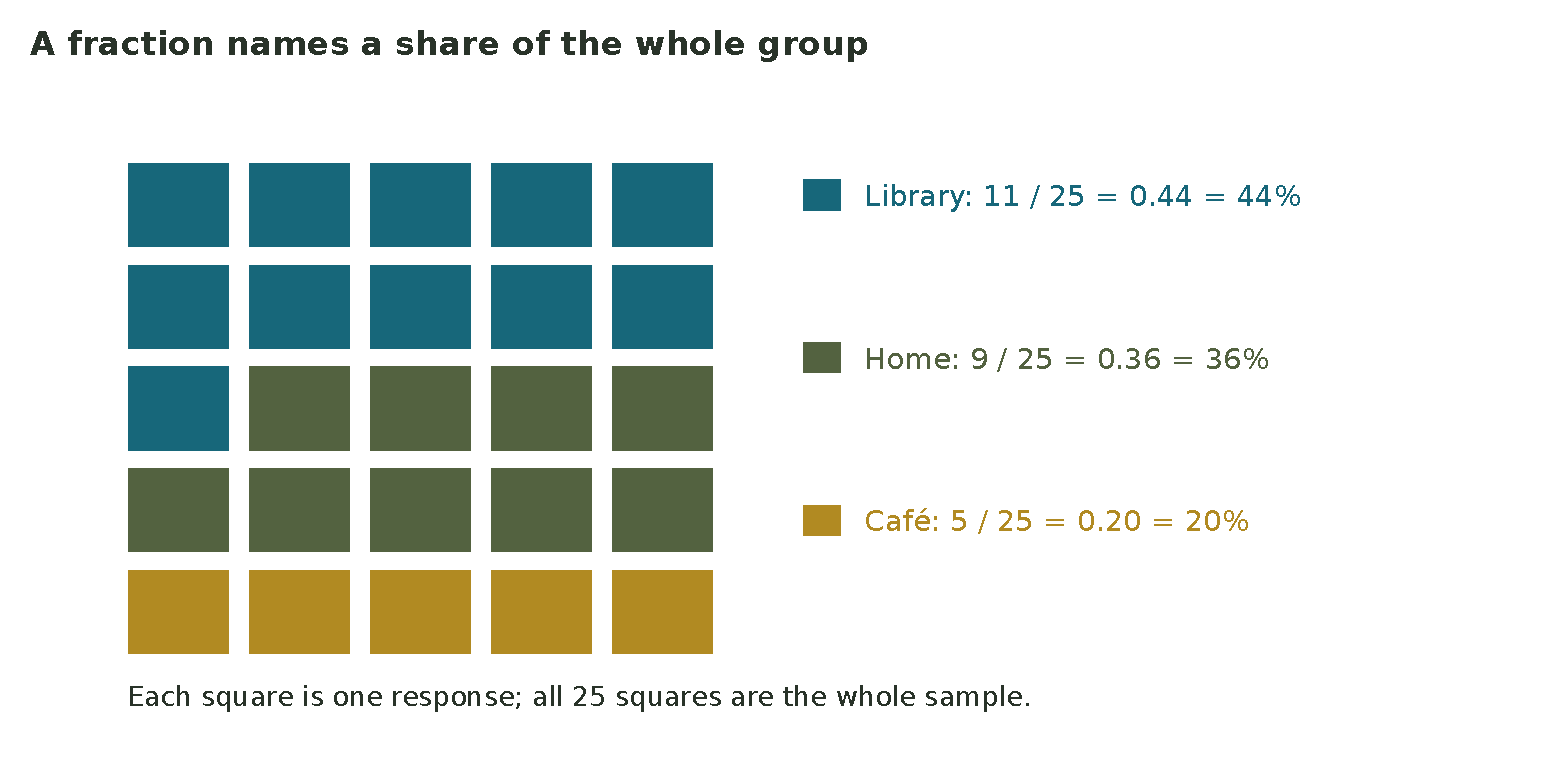
\includegraphics[width=\linewidth,height=2.8in,keepaspectratio]{../assets/week2/relative-frequency.pdf}\captionof*{figure}{A count, a fraction, a decimal, and a percentage can describe the same part of a whole.}\end{minipage}\par\medskip

\begin{tcolorbox}[title={What does a survey result mean?}]
If 11 of 25 respondents choose the library, the observed library share is 44\%. Extending that result to everyone at the college requires another question: who had a chance to be included, and who was missed?
\end{tcolorbox}
Week 1 used fractions as parts of a whole. This chapter uses that idea to organize observations, compare groups, read graphs, and describe probability models. We keep observed results separate from predictions about future trials or a larger population.

Try the short checks before reading their explanations. Additional examples follow the reading. The 26 practice and review groups retain the earlier chapter's datasets and questions, with corrections to ambiguous graph labels and sampling language. Complete solutions follow. The situations are hypothetical.

\medskip
\href{https://bobovski66.github.io/MathInSociety/readings/week2_reading.html}{Online reading}\quad\textperiodcentered\quad\href{https://bobovski66.github.io/MathInSociety/demos/probability_distribution.html}{Counts and chance explorer}\quad\textperiodcentered\quad\href{https://bobovski66.github.io/MathInSociety/labs/week2_lab.html}{Laboratory}
\clearpage

\Needspace{6\baselineskip}\section{Who or what are we trying to describe?}

Suppose a college wants to learn how students get to campus. It could ask everyone, but that may take too much time. Instead, it asks a smaller group. We call these groups the population and the sample.


The \emph{population} is the whole group we want to learn about. The \emph{sample} is the group actually observed. If a college has 1,600 enrolled students and asks 80 of them about their travel, the population is all 1,600 students. The sample is the 80 who answer.


A \emph{variable} is what we record for each observation: perhaps usual travel method or travel time in minutes. One person can supply both a category and a measurement.


\par\medskip\noindent\begin{minipage}{\linewidth}
\centering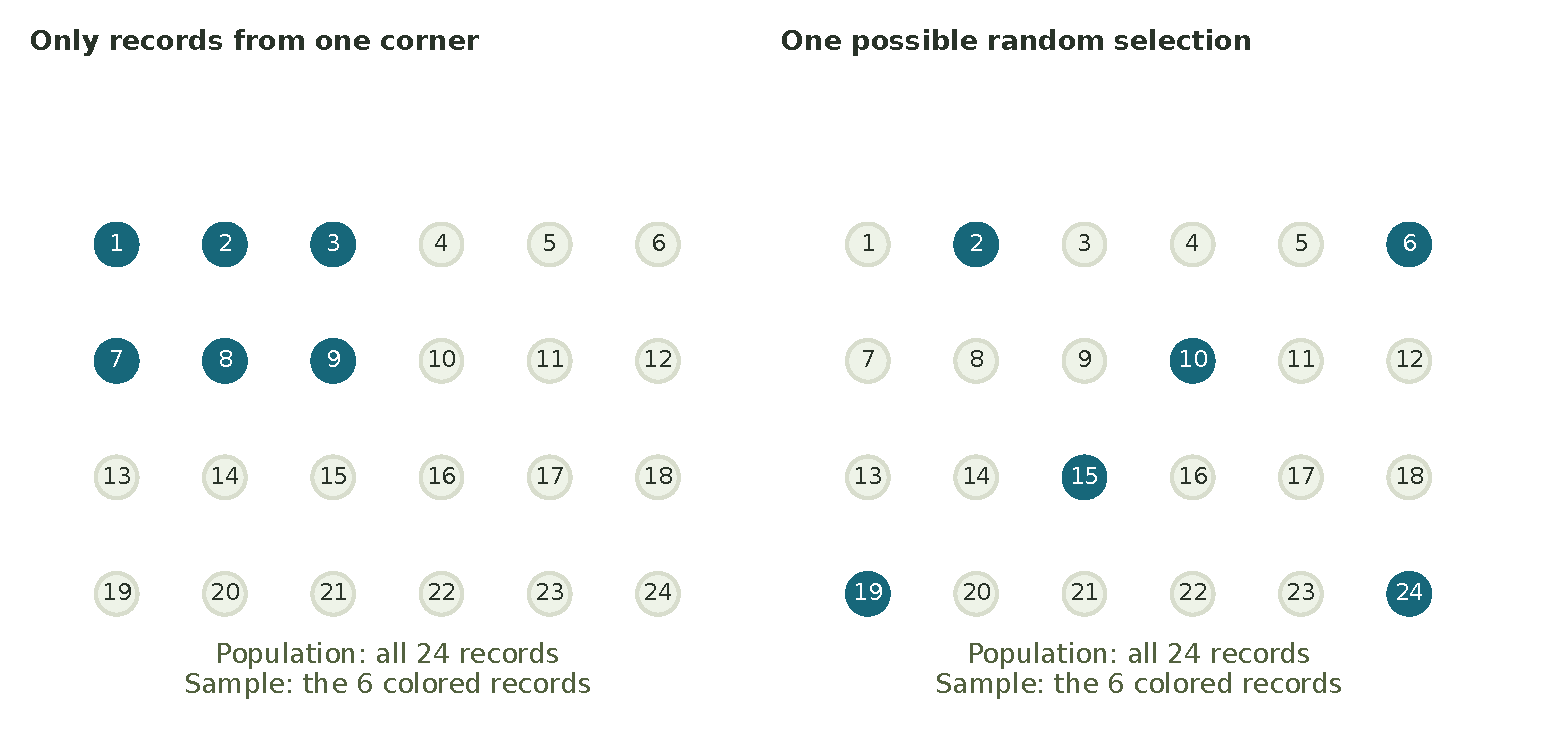
\includegraphics[width=\linewidth,height=2.65in,keepaspectratio]{../assets/week2/population-sample.pdf}
\captionof*{figure}{The way a sample is selected affects the result. The picture on the right shows one possible random selection.}
\end{minipage}\par\medskip

\begin{tcolorbox}[title={How the sample is selected},breakable]

Asking only people standing at the bicycle rack is likely to include many cyclists. Even 500 answers collected there could miss students who park elsewhere, arrive later, or study online.


For a \emph{simple random sample} of 80, every possible group of 80 students has the same chance of being chosen. One way is to use a complete student list and randomly choose 80 different names.


\end{tcolorbox}

Every sample gives only a partial view. Chance alone can make two random samples differ. A sampling method can also consistently favor some parts of the population; that is a source of \emph{sampling bias}. More answers from the same limited location do not automatically fix the problem. Also ask who did not respond.


\begin{tcolorbox}[title={Pause and try 1},breakable]
To learn about all library visits during a month, a researcher records visits on one Friday afternoon. Name the population, the sample, and one limitation.
\end{tcolorbox}

\Needspace{6\baselineskip}\section{Frequency: count how often each answer appears}

A \emph{frequency} is a count. A frequency table puts each answer beside the number of times it appears. The frequencies should total the number of responses.


\begin{tcolorbox}[title={One preferred study location per person},breakable]

Twenty-five students each choose one location. Eleven choose the library, nine choose home, and five choose a café.


\end{tcolorbox}

\par\medskip{\small\renewcommand{\arraystretch}{1.35}\begin{tabularx}{\linewidth}{@{}YY@{}}\toprule
Study location & Frequency\\
\midrule
Library & 11\\
Home & 9\\
Café & 5\\
Total & 25\\
\bottomrule\end{tabularx}}\par\medskip

The check is 11 + 9 + 5 = 25, matching the number of responses. Each student contributed one answer, so the counts add to 25.


Numbers can be answers too. For the pet counts 0, 1, 1, 2, 0, 1, the frequencies are 2 for zero pets, 3 for one pet, and 1 for two pets. Zero pets is a recorded answer; it is not a missing response.


\begin{tcolorbox}[title={When someone can choose more than one answer},breakable,colback=warm,colbacktitle=warm,coltitle=gold,colframe=gold!35]

If a survey allows multiple answers, a person can appear in more than one category. In our examples, each person selects one answer.


\end{tcolorbox}

\begin{tcolorbox}[title={Pause and try 2},breakable]
For the answers red, blue, red, green, blue, red, make a frequency table and check its total.
\end{tcolorbox}

\Needspace{6\baselineskip}\section{Relative frequency: what share of the whole?}

A count tells us how many. A \emph{relative frequency} tells us what fraction of the observations fall in a category. Divide that category's count by the total number of observations.

\[\text{relative frequency}=\frac{\text{category count}}{\text{total count}}.\]
The denominator is the total number of observations. For the library, divide 11 by 25: 11/25 = 0.44. Multiply the decimal by 100 to get 44\%. All three represent the same share of the sample.


\par\medskip\noindent\begin{minipage}{\linewidth}
\centering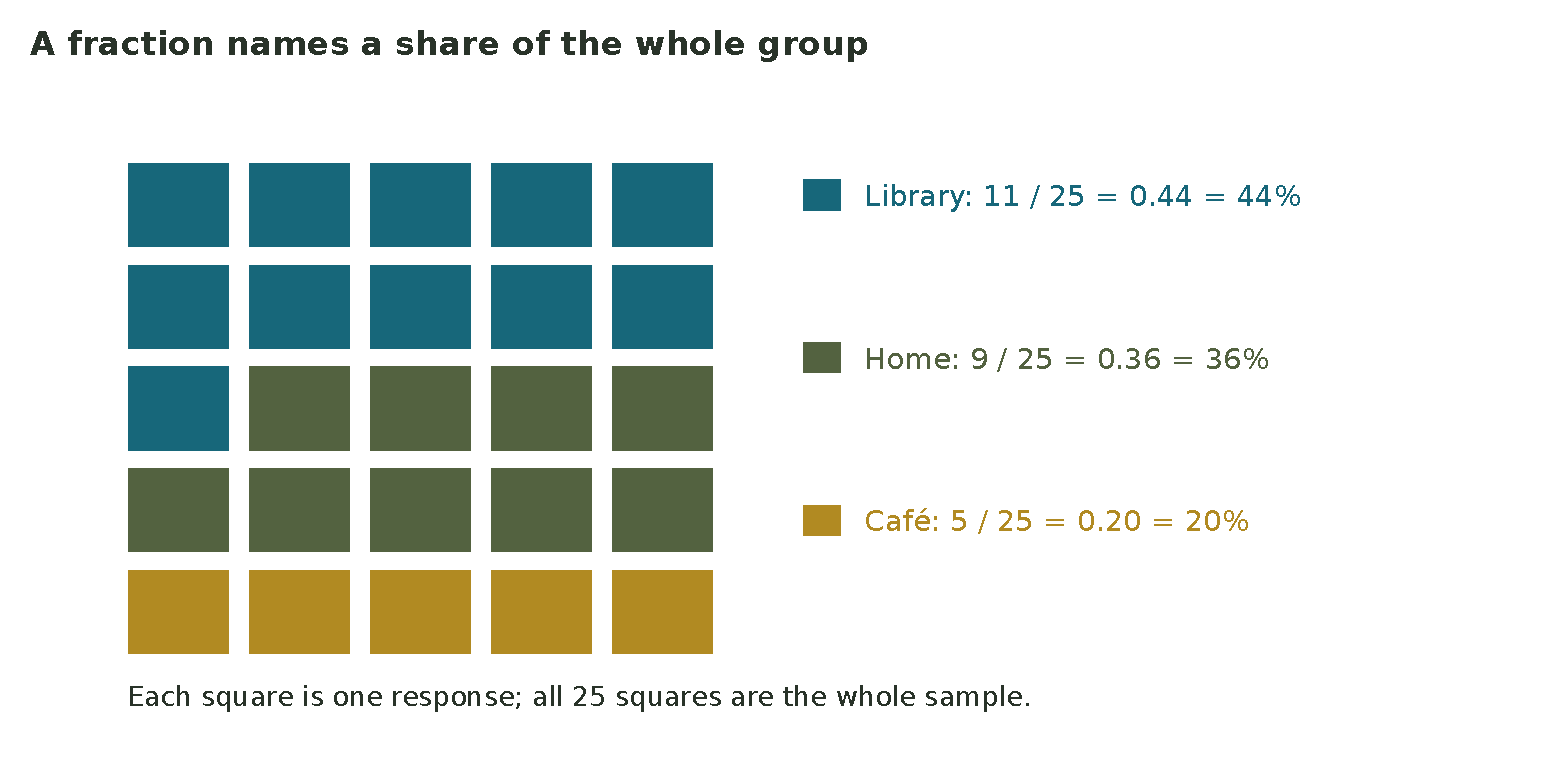
\includegraphics[width=\linewidth,height=2.65in,keepaspectratio]{../assets/week2/relative-frequency.pdf}
\captionof*{figure}{Each category uses the same total of 25 responses.}
\end{minipage}\par\medskip

\par\medskip{\small\renewcommand{\arraystretch}{1.35}\begin{tabularx}{\linewidth}{@{}YYYY@{}}\toprule
Location & Fraction & Decimal & Percentage\\
\midrule
Library & 11/25 & 0.44 & 44\%\\
Home & 9/25 & 0.36 & 36\%\\
Café & 5/25 & 0.20 & 20\%\\
Total & 25/25 & 1 & 100\%\\
\bottomrule\end{tabularx}}\par\medskip

The exact fractions add to 1 because all 25 answers are included once. Rounded decimals may add to something like 0.999 instead. For exact calculations, use the fractions before rounding. If the sample has no observations, there is no relative frequency to calculate: division by zero does not give a share.


\begin{tcolorbox}[title={Pause and try 3},breakable]
Eight of 40 recorded answers are in one category. Write its share as a fraction, decimal, and percentage.
\end{tcolorbox}

\Needspace{6\baselineskip}\section{Why totals matter when comparing groups}

Suppose 6 of 10 people in one group answer yes, while 12 of 30 in another group answer yes. The second group has more yes answers, but it is also three times as large.


\begin{tcolorbox}[title={Comparing the proportions},breakable]

First group: 6/10 = 0.60 = 60\%. Second group: 12/30 = 0.40 = 40\%. Yes is more common as a share of the first group, even though the second group has more yes answers.


\end{tcolorbox}

\par\medskip\noindent\begin{minipage}{\linewidth}
\centering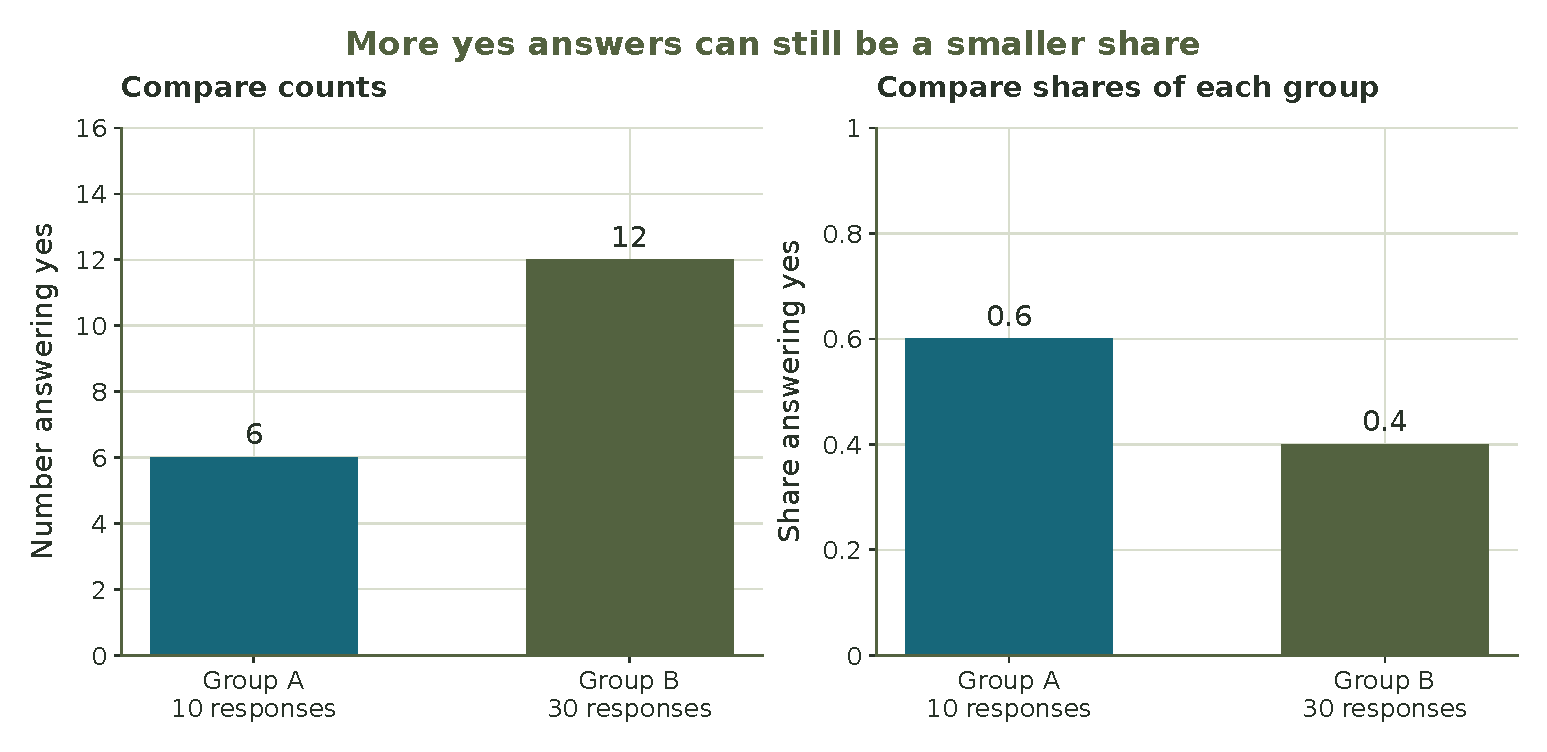
\includegraphics[width=\linewidth,height=2.65in,keepaspectratio]{../assets/week2/sample-size-comparison.pdf}
\captionof*{figure}{The second group has more yes answers, but the first has a higher percentage of yes answers.}
\end{minipage}\par\medskip

When group sizes differ, relative frequencies make comparisons more useful. The way each group was selected still matters.


\begin{tcolorbox}[title={Pause and try 4},breakable]
One survey has 9 yes answers out of 15; another has 18 out of 30. Which has the larger yes share?
\end{tcolorbox}

\Needspace{6\baselineskip}\section{Choose a graph that matches the data}

A \emph{bar chart} compares separate categories, such as library, home, and café. Each bar's height shows a count or a relative frequency. The bars are separated because the categories are distinct.


A \emph{histogram} groups numerical observations into intervals, called \emph{bins}. For travel time, bins might be 0 to under 10 minutes, 10 to under 20, and so on. Adjacent bins sit next to each other on a number scale, so their bars touch.


\par\medskip\noindent\begin{minipage}{\linewidth}
\centering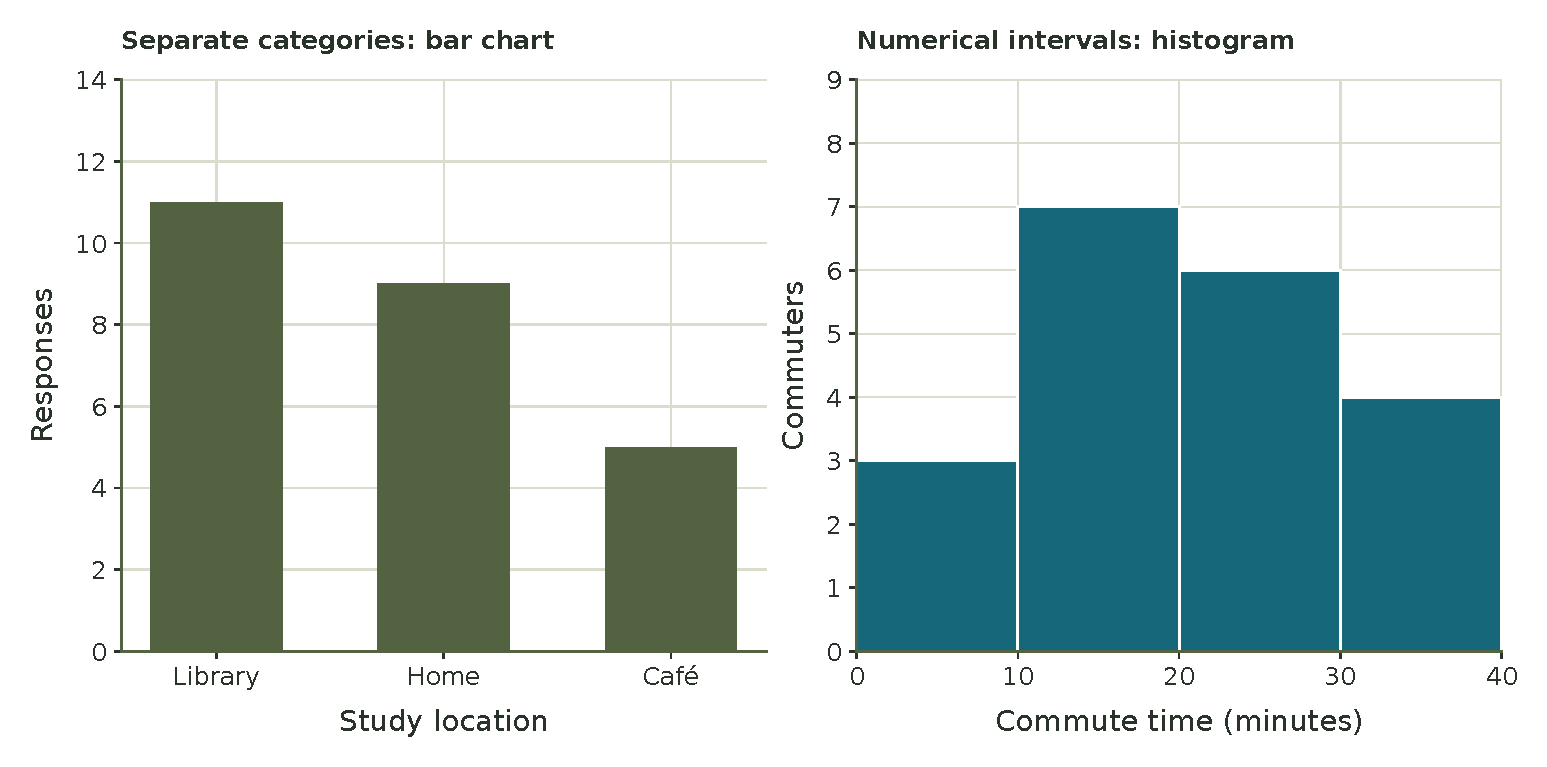
\includegraphics[width=\linewidth,height=2.65in,keepaspectratio]{../assets/week2/bar-and-histogram.pdf}
\captionof*{figure}{Check whether the vertical axis shows counts or proportions.}
\end{minipage}\par\medskip

A bar chart's categories can often be rearranged. Histogram intervals follow numerical order. For a few separate numerical counts, such as books read, a bar chart can also be useful. Use a histogram when the task asks you to group measurements into intervals.


Bar-chart heights should be measured from zero for a fair visual comparison. In this chapter, histogram bins have equal widths; their heights can therefore directly show counts or relative frequencies. Unequal-width bins need additional care and are outside these exercises.


\begin{tcolorbox}[title={Pause and try 5},breakable]
Which display fits preferred lunch location? Which fits commuting time grouped into 15-minute intervals?
\end{tcolorbox}

\Needspace{6\baselineskip}\section{Reading histogram intervals}

The bin \([20,25)\) means ``20 up to, but not including, 25.'' The square bracket includes the endpoint; the parenthesis leaves it out.

\[20\le x<25.\]
Here x stands for one recorded value. The symbols say that x is at least 20 and less than 25. A value of 25 goes into the next bin, \([25,30)\). This rule prevents counting a boundary value twice.


\par\medskip\noindent\begin{minipage}{\linewidth}
\centering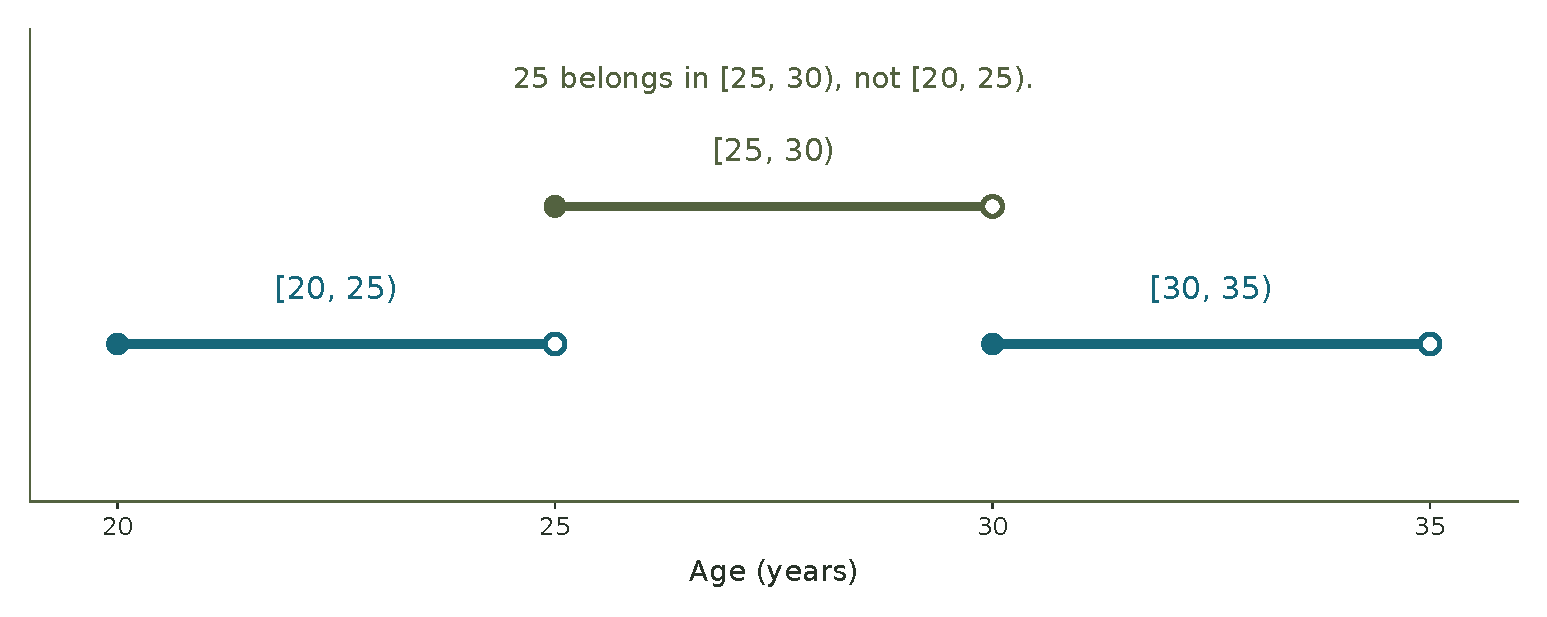
\includegraphics[width=\linewidth,height=2.65in,keepaspectratio]{../assets/week2/bin-boundaries.pdf}
\captionof*{figure}{These boundaries place each value in one interval. An interval can also have no observations.}
\end{minipage}\par\medskip

\begin{tcolorbox}[title={Placing values in bins},breakable]

For times 4, 9, 10, 16, 22, and 29 minutes, the bins [0,10), [10,20), [20,30) each contain two observations. The value 10 belongs in the second bin.


\end{tcolorbox}

The same data can look quite different with wider or narrower bins. Bin widths are worth checking when comparing two histograms.


\begin{tcolorbox}[title={Pause and try 6},breakable]
Where do 29, 30, and 35 belong in the bins [25,30), [30,35), [35,40)?
\end{tcolorbox}

\Needspace{6\baselineskip}\section{From observed shares to a model of chance}

When we randomly choose one answer from the 25 study-location responses, the chance of choosing a library answer is exactly 11/25. When we use that share to describe all students at the college, it is an estimate. Its usefulness depends on how well the survey reaches that larger group.


Probability can also come from a stated mathematical model rather than a survey. For example, a bag contains 4 red, 3 blue, and 5 green marbles. Assume each individual marble is equally likely to be drawn.


\par\medskip\noindent\begin{minipage}{\linewidth}
\centering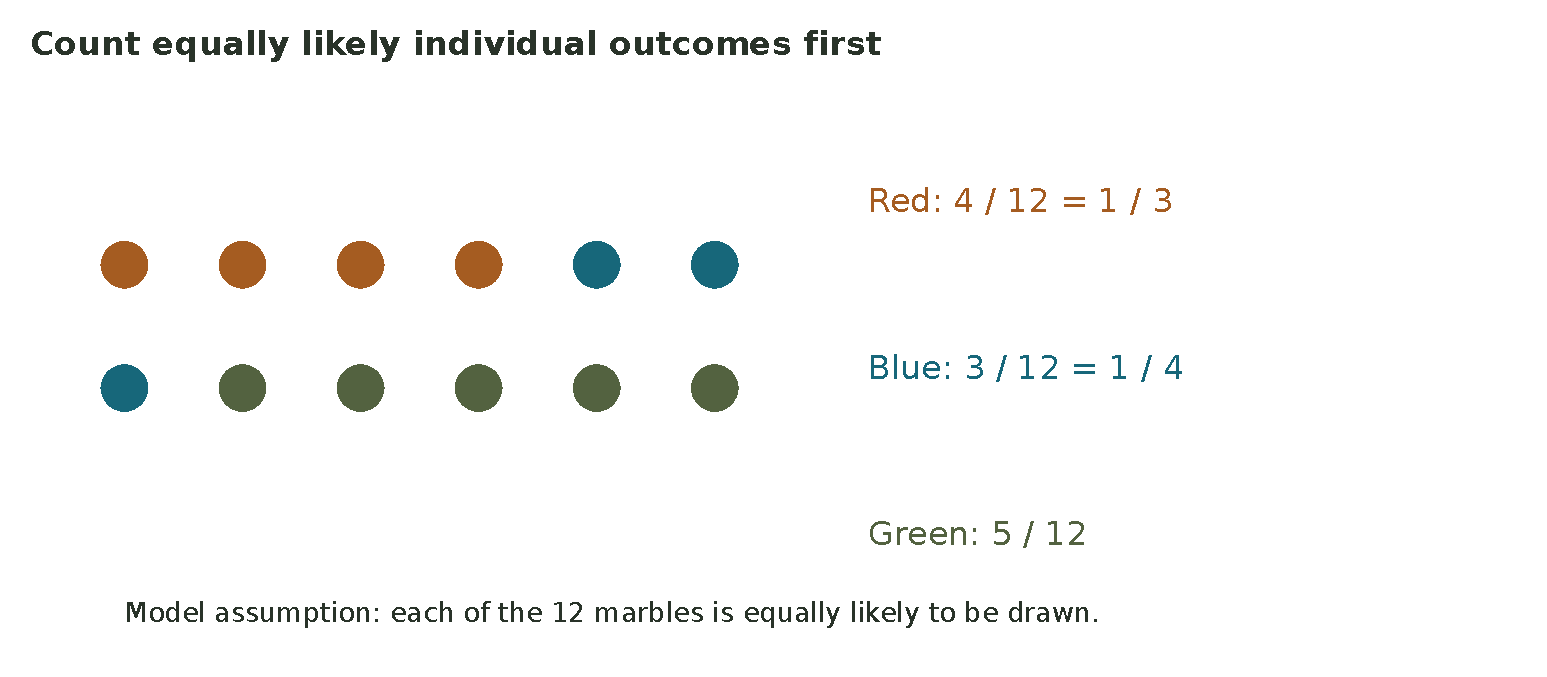
\includegraphics[width=\linewidth,height=2.65in,keepaspectratio]{../assets/week2/marble-model.pdf}
\captionof*{figure}{Each marble has the same chance of being drawn; colors with more marbles have higher probabilities.}
\end{minipage}\par\medskip

\begin{tcolorbox}[title={Counting the marbles},breakable]

There are 12 marbles in all. The model gives P(red) = 4/12 = 1/3, P(blue) = 3/12 = 1/4, and P(green) = 5/12. The letter P means ``probability of.'' The words inside parentheses say which outcome we mean.


\end{tcolorbox}

An \emph{empirical} distribution comes from observed counts. A \emph{theoretical} distribution comes from a model's assumptions, such as equal chances for a fair die. We can compare the two, but they answer different questions: what happened and what the model predicts.


\begin{tcolorbox}[title={Pause and try 7},breakable]
A fair die assigns probability 1/6 to a four. In 12 actual rolls, four appears once. Are the model probability and observed relative frequency the same number?
\end{tcolorbox}

\Needspace{6\baselineskip}\section{A probability distribution accounts for every possibility}

A \emph{probability distribution} lists possible outcomes and gives each a probability. For the finite lists in this week's work, two rules matter: every probability lies between 0 and 1, and all the probabilities add to 1.


The outcomes must cover every possibility without overlap. For one spin labeled A, B, or C, exactly one of those outcomes occurs. If their probabilities are 0.20, 0.30, and 0.50, the total is 1.


\par\medskip{\small\renewcommand{\arraystretch}{1.35}\begin{tabularx}{\linewidth}{@{}YYY@{}}\toprule
Outcome & Probability & Meaning in the model\\
\midrule
A & 0.20 & 20\% of the probability\\
B & 0.30 & 30\% of the probability\\
C & 0.50 & 50\% of the probability\\
Total & 1.00 & All possibilities\\
\bottomrule\end{tabularx}}\par\medskip

Within this finite model, 0 assigns no chance to an outcome and 1 assigns all the chance. But seeing zero occurrences in a small sample does not establish that an outcome is impossible in the real process.


\begin{tcolorbox}[title={Finding a missing probability},breakable]

Suppose three outcomes have probabilities 0.18, 0.47, and p. The first two use 0.65 of the total. The missing probability is p = 1 $-$ 0.65 = 0.35.


\end{tcolorbox}

The notation \(p_i\) represents the probability of outcome i. The expression \(\sum p_i=1\) means that the probabilities of all outcomes add to 1.


\begin{tcolorbox}[title={Pause and try 8},breakable]
Can 0.45, 0.35, and 0.30 form the complete probability distribution for three separate outcomes?
\end{tcolorbox}

\Needspace{6\baselineskip}\section{Events, ``or,'' and ``not''}

An \emph{event} can include several outcomes. For a die, ``an even result'' includes 2, 4, and 6. Add probabilities when the listed alternatives cannot happen together on the same trial.


\begin{tcolorbox}[title={Example: even results on a die},breakable]

For one fair die, P(even) = P(2) + P(4) + P(6) = 3/6 = 1/2. A single roll cannot be both 2 and 4, so these outcomes do not overlap.


\end{tcolorbox}

The \emph{complement} of an event is everything outside it: ``not that event.'' Together, an event and its complement cover the whole probability.

\[P(\text{not }A)=1-P(A).\]
\par\medskip\noindent\begin{minipage}{\linewidth}
\centering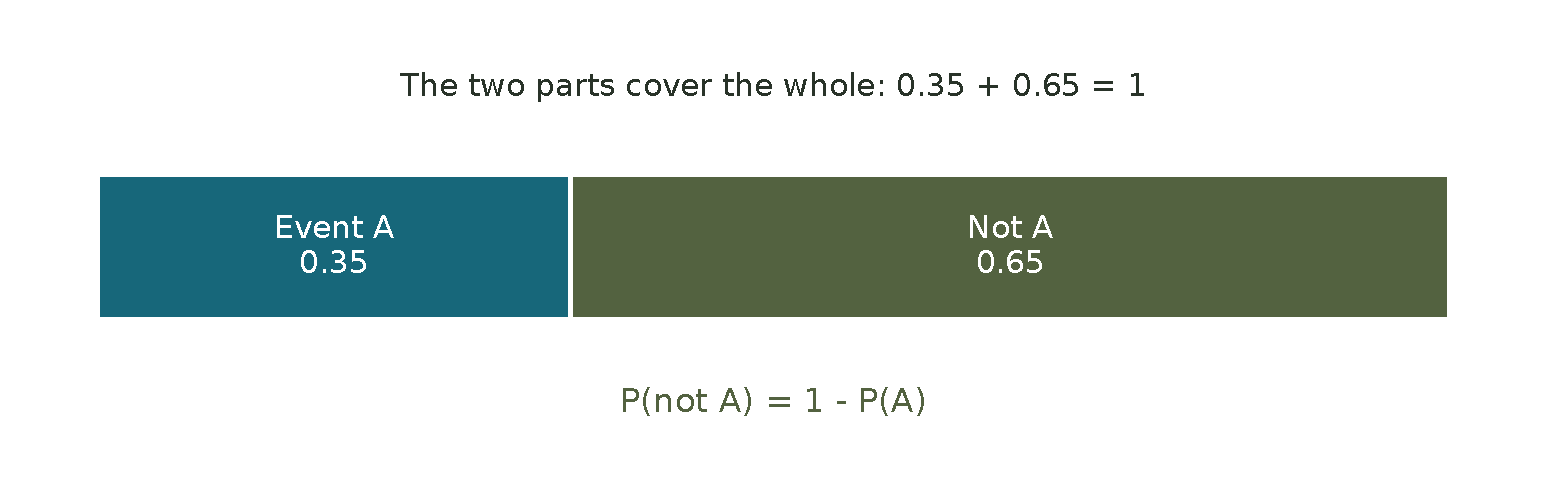
\includegraphics[width=\linewidth,height=2.65in,keepaspectratio]{../assets/week2/probability-complement.pdf}
\captionof*{figure}{The complement accounts for all outcomes outside the event.}
\end{minipage}\par\medskip

\begin{tcolorbox}[title={An 'at least one' probability},breakable]

If P(zero late deliveries) = 0.60, then P(at least one late delivery) = 1 $-$ 0.60 = 0.40. We can calculate this by subtracting the probability of zero late deliveries from 1.


\end{tcolorbox}

Some events overlap. For example, 'even' and 'greater than 3' both include 4 and 6. Those outcomes count only once when finding the probability of either event.


\begin{tcolorbox}[title={Pause and try 9},breakable]
For one fair die, find the probability of 1 or 2, then the probability of neither 1 nor 2.
\end{tcolorbox}

\Needspace{6\baselineskip}\section{Counting outcomes with two dice}

Assume two fair six-sided dice are rolled independently: the result of one does not change the chances for the other. Imagine one die is red and the other blue so we can keep their roles separate.


There are 6 choices for the first die and 6 for the second, giving 6 $\times$ 6 = 36 equally likely ordered pairs. The pair (1,6) is different from (6,1), even though both have sum 7.


\par\medskip\noindent\begin{minipage}{\linewidth}
\centering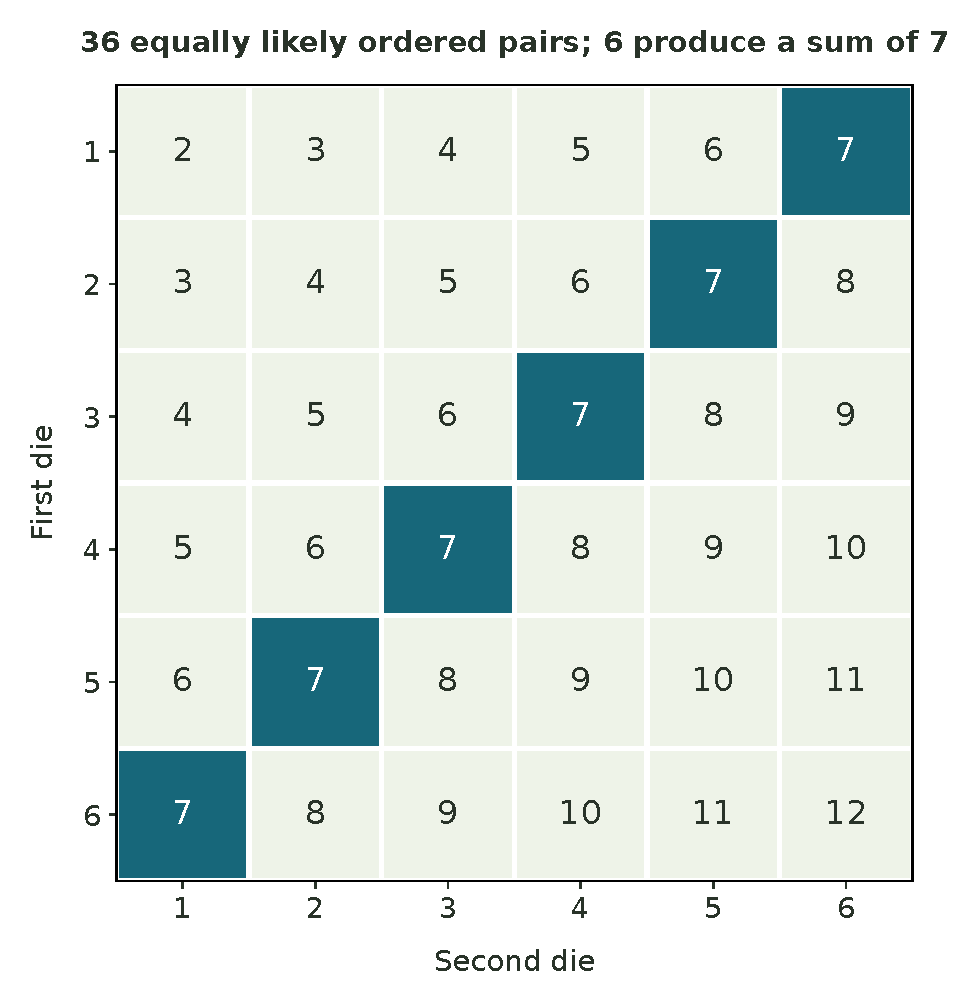
\includegraphics[width=\linewidth,height=3.8in,keepaspectratio]{../assets/week2/dice-outcomes.pdf}
\captionof*{figure}{Each cell has probability 1/36. Several different cells can lead to the same sum.}
\end{minipage}\par\medskip

\begin{tcolorbox}[title={Probabilities of the sums},breakable]

A sum of 2 comes only from (1,1), so its probability is 1/36. A sum of 7 comes from six pairs: (1,6), (2,5), (3,4), (4,3), (5,2), (6,1). Its probability is 6/36 = 1/6.


\end{tcolorbox}

\par\medskip\noindent\begin{minipage}{\linewidth}
\centering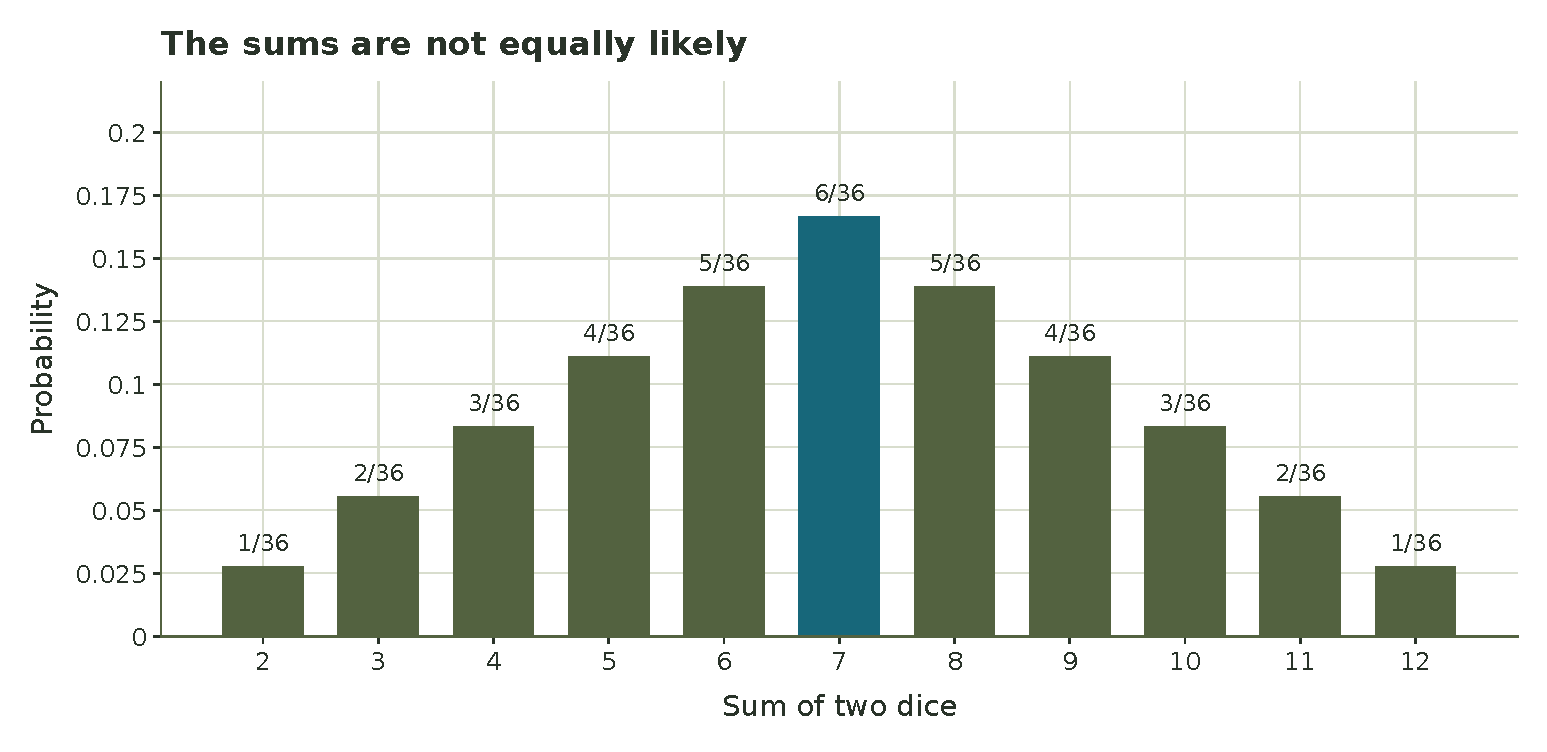
\includegraphics[width=\linewidth,height=2.65in,keepaspectratio]{../assets/week2/dice-distribution.pdf}
\captionof*{figure}{Group the 36 equally likely pairs by their sums. The resulting distribution is symmetric around 7.}
\end{minipage}\par\medskip

\begin{tcolorbox}[title={Pause and try 10},breakable]
How many pairs produce a sum of 11, and what is its probability?
\end{tcolorbox}

\Needspace{6\baselineskip}\section{Probability over repeated trials}

For a fair coin, heads and tails each have probability 0.50. Ten flips may produce more or fewer than five heads, including several heads in a row.


In repeated independent trials with the same probabilities, relative frequencies tend to settle closer to the model probabilities as the number of trials grows. They can still move farther away at a particular step. After a run of heads, a fair independent coin still has probability 0.50 of heads on the next flip.


\par\medskip\noindent\begin{minipage}{\linewidth}
\centering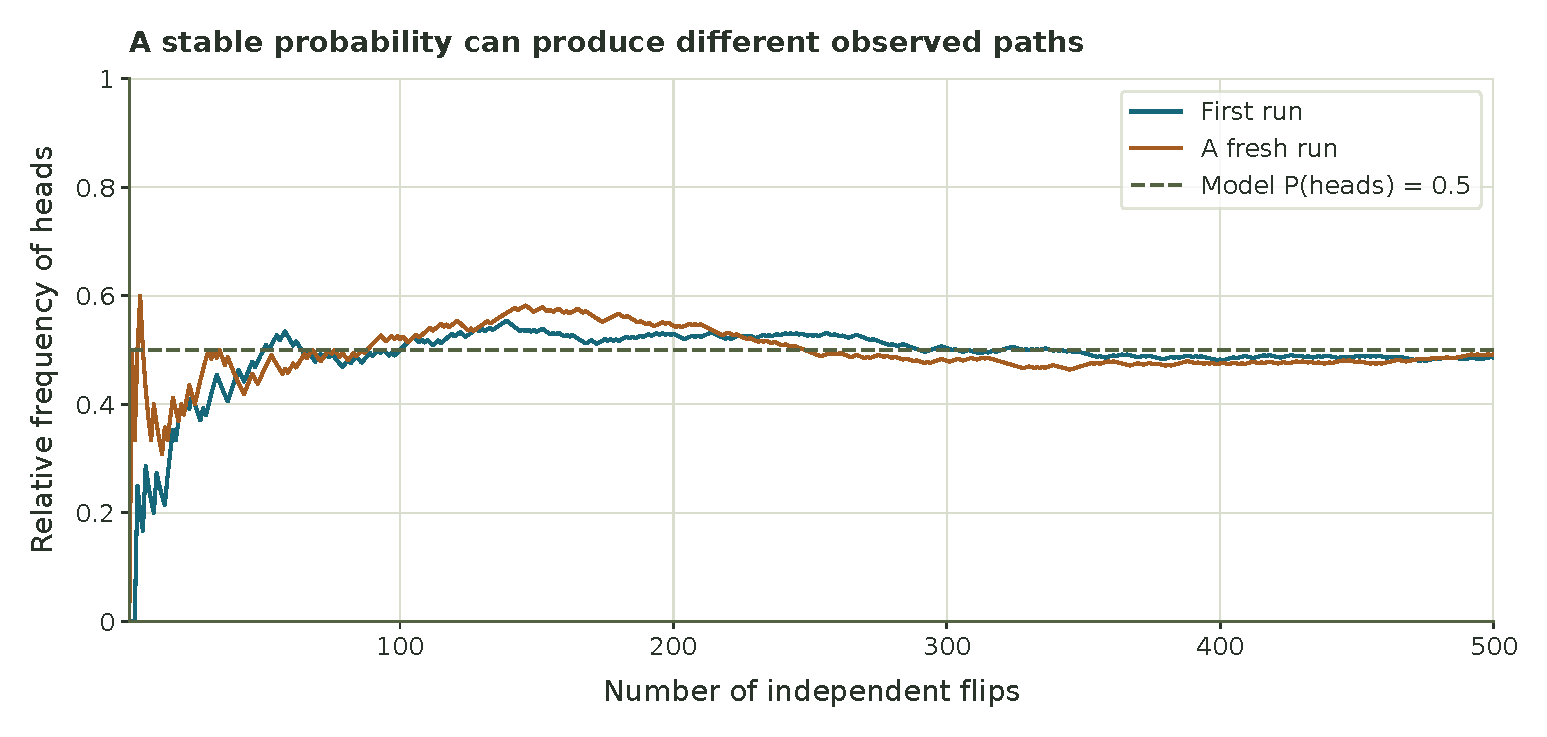
\includegraphics[width=\linewidth,height=2.65in,keepaspectratio]{../assets/week2/repeated-trials.pdf}
\captionof*{figure}{The probability of heads stays at 0.50, while the observed proportion changes with each new flip.}
\end{minipage}\par\medskip

\begin{tcolorbox}[title={Expected counts},breakable]

If a fixed process has probability 0.30 of a particular outcome, then across 200 trials its \emph{expected count} is 200 $\times$ 0.30 = 60. The expected count is 60, though an individual run may have a different count.


\end{tcolorbox}

The repeated-trial explorer keeps a model fixed while drawing new observations. Compare the model's probabilities with the sample's counts and shares. The next-token application uses the same idea for possible continuations of text.


\begin{tcolorbox}[title={Pause and try 11},breakable]
A fixed model gives an outcome probability 0.10. What count is expected in 50 independent trials? Must the actual count equal it?
\end{tcolorbox}

\Needspace{6\baselineskip}\section{Interpreting a distribution}

A distribution describes how observations or probability are spread across possibilities. For numerical data, look for where values cluster, how widely they spread, and which direction a tail extends.


\par\medskip\noindent\begin{minipage}{\linewidth}
\centering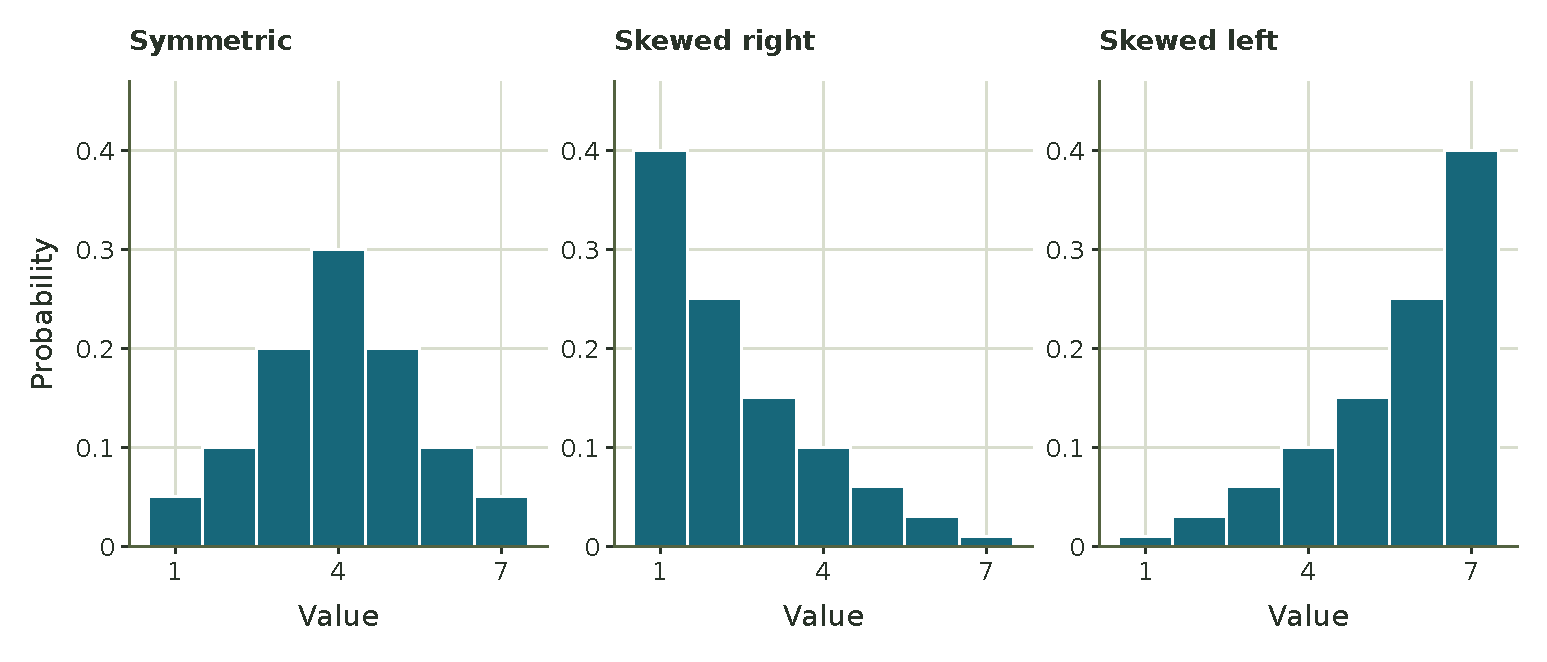
\includegraphics[width=\linewidth,height=2.65in,keepaspectratio]{../assets/week2/distribution-shapes.pdf}
\captionof*{figure}{Skew is named for the direction of the longer tail.}
\end{minipage}\par\medskip

The tallest bar identifies a most common category or interval. That interval may contain less than half the observations. Week 3 develops different ways to describe a center and a spread.


\begin{tcolorbox}[title={What a survey result tells us},breakable,colback=warm,colbacktitle=warm,coltitle=gold,colframe=gold!35]

``Eleven students chose the library'' reports a count. ``44\% of these respondents chose the library'' reports a sample share. ``We estimate that 44\% of all students prefer the library'' makes a claim about a larger population. Whether the last estimate is useful depends on how the students were sampled.


\end{tcolorbox}

Before using a distribution to make a decision, ask what the observations describe, who or what is missing, what the denominator means, and which parts come from assumptions. The discussion asks you to apply those questions to a survey you would care about.


\begin{tcolorbox}[title={Pause and try 12},breakable]
A category is the tallest bar at 40\%. Is it a majority? What extra information would you want before applying that share to a whole town?
\end{tcolorbox}

\subsection*{Activities and further reading}
Use the \href{https://bobovski66.github.io/MathInSociety/demos/probability_distribution.html}{explorer} to distinguish observed counts and shares from a fixed model. The \href{https://bobovski66.github.io/MathInSociety/applications/week2_application.html}{transportation application} uses 80 survey responses; the \href{https://bobovski66.github.io/MathInSociety/applications/week2_ai.html}{next-token application} uses a four-outcome model for repeated draws. The \href{https://bobovski66.github.io/MathInSociety/discussions/week2_discussion.html}{discussion} asks you to design a survey about something that matters to you.

OpenStax provides additional explanations of \href{https://openstax.org/books/introductory-statistics-2e/pages/1-2-data-sampling-and-variation-in-data-and-sampling}{data and sampling} and \href{https://openstax.org/books/introductory-statistics-2e/pages/2-2-histograms-frequency-polygons-and-time-series-graphs}{histograms}. The AI activities refer to Hugging Face's \href{https://huggingface.co/docs/transformers/generation_strategies}{generation strategies} for the distinction between sampling and choosing a most probable token.

\Needspace{8\baselineskip}
\section*{More worked examples}
\subsection*{A selection plan needs a population}
A school surveys one advisory class to learn about all students in the school. The school is the population; that advisory class is the sample. If the advisory contains only seniors, other grade levels are missing. Asking more students from the same advisory does not solve that coverage problem.

A biologist weighs 50 fish caught at randomly chosen locations in a lake. The intended population is all fish in the lake; the observed sample is the 50 captured fish. Spreading locations can reach different habitats, but it does not automatically give every fish an equal chance of being caught. The gear and the fish's behavior can matter too.

\subsection*{Count defects before calculating shares}
For 20 inspected products, the recorded numbers of defects are
\begin{quote}0, 1, 0, 2, 1, 0, 1, 3, 0, 1, 2, 0, 1, 0, 1, 0, 2, 1, 0, 1.\end{quote}
\par\medskip{\small\renewcommand{\arraystretch}{1.25}\begin{tabularx}{\linewidth}[t]{@{}YYYY@{}}\toprule
Outcome & Frequency & Fraction & Decimal\\\midrule
{0} & 8 & $\frac{2}{5}$ & 0.4000\\
{1} & 8 & $\frac{2}{5}$ & 0.4000\\
{2} & 3 & $\frac{3}{20}$ & 0.1500\\
{3} & 1 & $\frac{1}{20}$ & 0.0500\\
Total & 20 & 1 & 1.0000\\\bottomrule\end{tabularx}}\par\medskip

Both zero defects and one defect occur eight times. The sample share with at least one defect is $(8+3+1)/20=12/20=0.60$. Equivalently, subtract the zero-defect share from 1: $1-8/20=0.60$. These calculations describe the inspected items.

\Needspace{8\baselineskip}
\subsection*{Read a category bar chart}

\par\medskip\noindent\begin{minipage}{\linewidth}\centering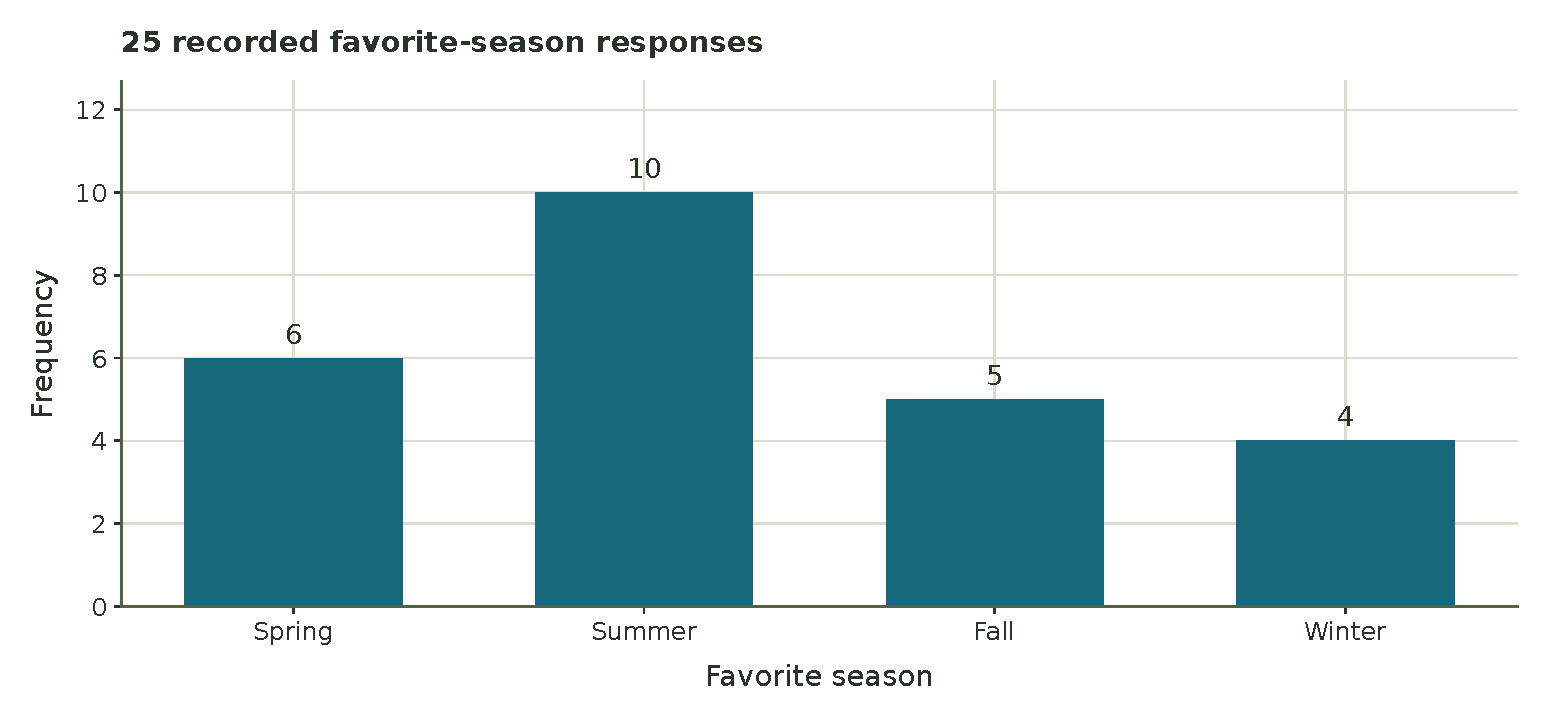
\includegraphics[width=\linewidth,height=2.6in,keepaspectratio]{../assets/week2/seasons.pdf}\captionof*{figure}{The recorded counts total 25. Summer has the largest count, 10; this is 40\%, not a majority.}\end{minipage}\par\medskip

The share preferring Fall is $5/25=0.20$. The probability is exactly 0.20 when we choose uniformly from these 25 responses. Applying it to all students would be an estimate requiring information about how the respondents were selected.

\Needspace{8\baselineskip}
\subsection*{Check a table against its raw data}
The business records calls on 30 days:
\begin{quote}5, 8, 6, 7, 9, 5, 6, 8, 7, 6, 7, 8, 5, 9, 7, 6, 8, 7, 6, 5, 8, 7, 6, 9, 7, 8, 6, 7, 5, 8.\end{quote}
\par\medskip{\small\renewcommand{\arraystretch}{1.25}\begin{tabularx}{\linewidth}[t]{@{}YYYY@{}}\toprule
Outcome & Frequency & Fraction & Decimal\\\midrule
{5} & 5 & $\frac{1}{6}$ & 0.1667\\
{6} & 7 & $\frac{7}{30}$ & 0.2333\\
{7} & 8 & $\frac{4}{15}$ & 0.2667\\
{8} & 7 & $\frac{7}{30}$ & 0.2333\\
{9} & 3 & $\frac{1}{10}$ & 0.1000\\
Total & 30 & 1 & 1.0000\\\bottomrule\end{tabularx}}\par\medskip

\par\medskip\noindent\begin{minipage}{\linewidth}\centering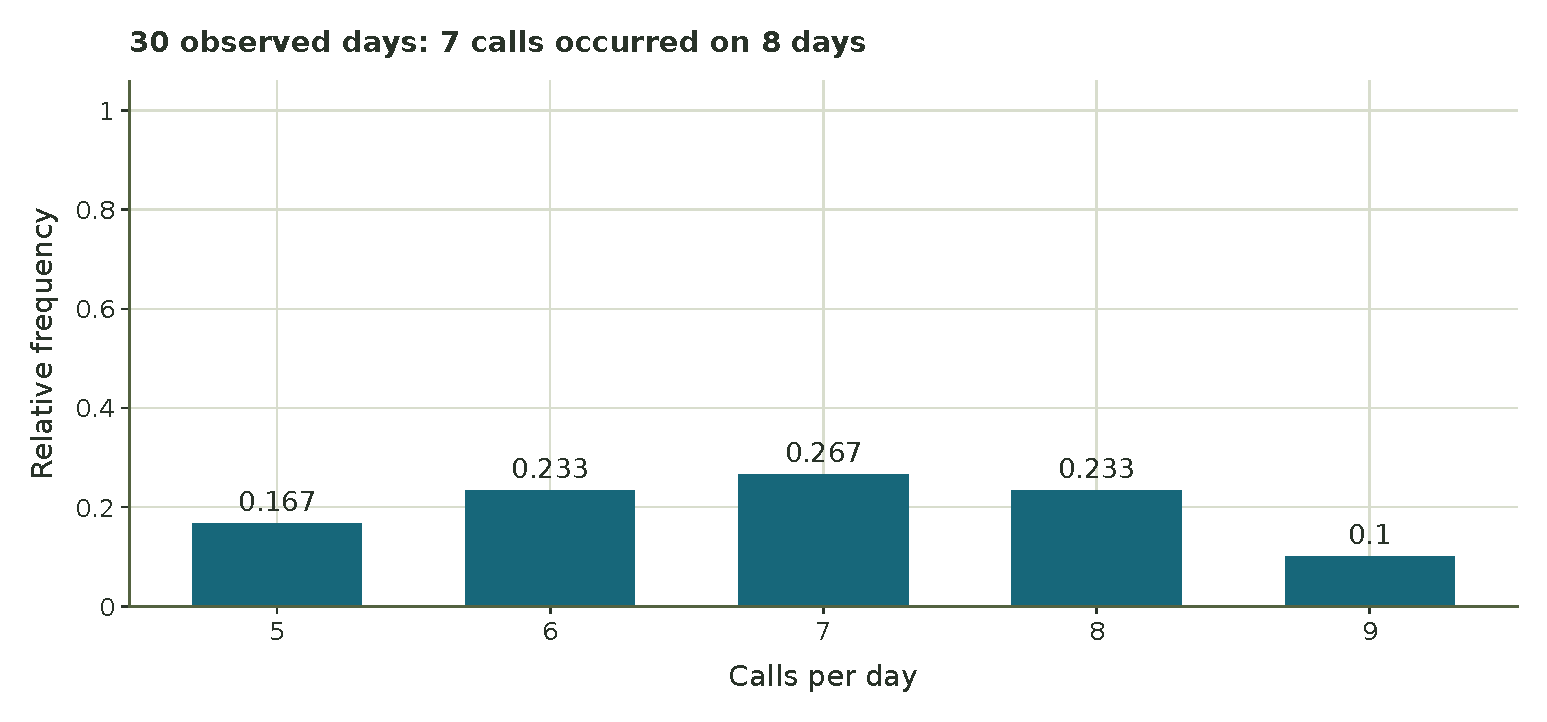
\includegraphics[width=\linewidth,height=2.6in,keepaspectratio]{../assets/week2/daily-calls.pdf}\captionof*{figure}{The most common observed count is 7 calls, on 8 of the 30 days. The fractions account for exactly 30 days.}\end{minipage}\par\medskip

The table must agree with the list, not just look plausible. Treating these proportions as predictions for future days assumes that the conditions remain relevant. An observed peak does not guarantee the next day's count.

\Needspace{8\baselineskip}
\subsection*{Read grouped quiz scores carefully}

\par\medskip\noindent\begin{minipage}{\linewidth}\centering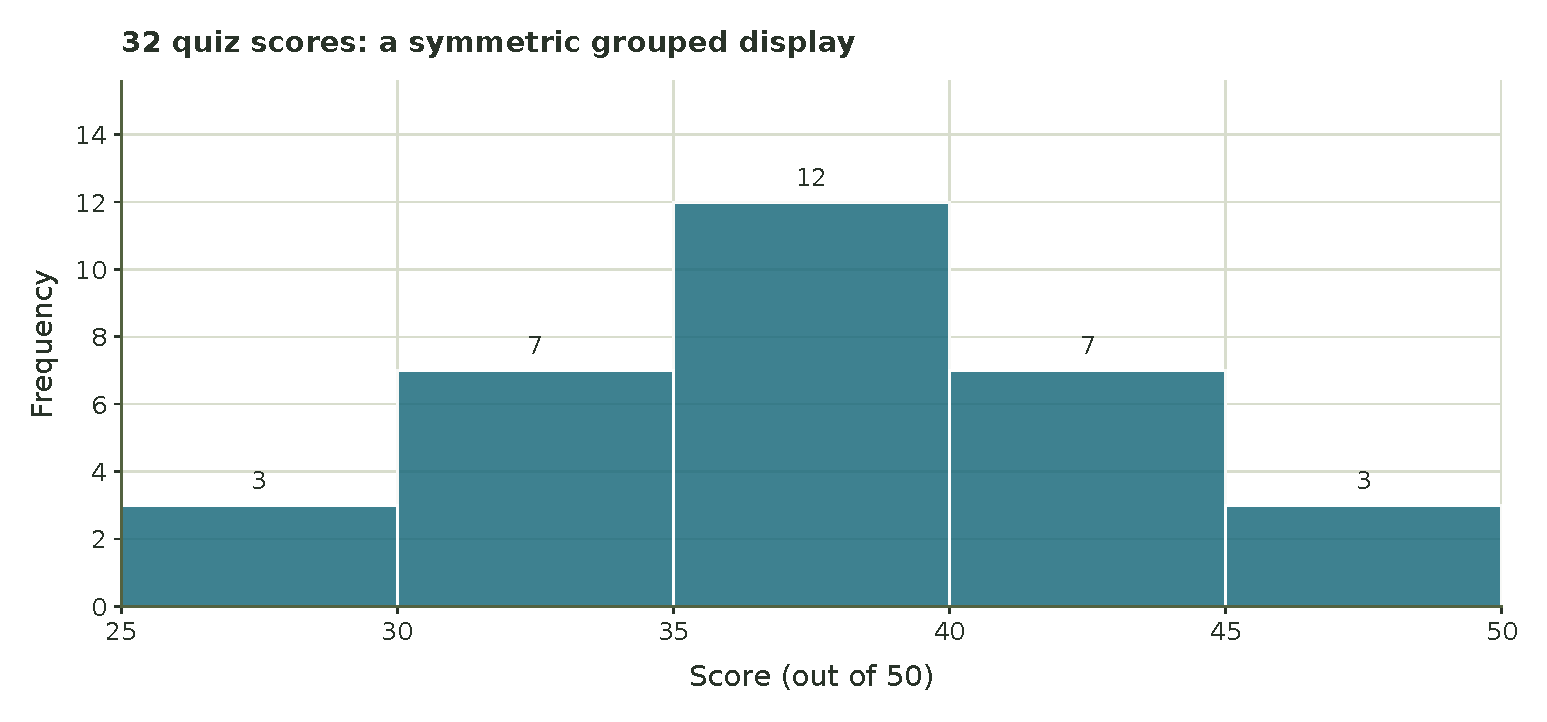
\includegraphics[width=\linewidth,height=2.6in,keepaspectratio]{../assets/week2/quiz-scores.pdf}\captionof*{figure}{Bins are [25,30), [30,35), [35,40), [40,45), and [45,50]. The final bin includes 50, the highest possible score.}\end{minipage}\par\medskip

The five counts are 3, 7, 12, 7, and 3, totaling 32 students. The tallest bin is [35,40), and the bin heights form a symmetric pattern. We know each score's interval, but not every exact score. These bars do not determine the exact average or prove that the raw scores are perfectly symmetric.
\clearpage
\section*{Practice A: Populations and samples}
These are the chapter's original practice situations. Name the group of interest before discussing what the selection method may miss.
\begin{enumerate}[label=A\arabic*.,leftmargin=2.5em,itemsep=10pt]
\item For each situation, identify the population and sample. Explain which parts of the population the sampling method might overrepresent or underrepresent.
\begin{enumerate}[label=(\alph*)]
\item A hospital uses ER patients from last Tuesday to estimate the average wait time for the whole month.
\item A polling organization calls 1,000 randomly selected registered voters to estimate support for a ballot measure.
\item A coffee shop asks only Monday-morning customers whether the shop should open earlier.
\end{enumerate}
\item A researcher wants to estimate daily screen time for teenagers in a city. Describe a simple random sampling plan, assuming a complete list is available. Describe a plan that would systematically favor part of the population.
\item Explain in two sentences why a larger sample does not automatically correct a problem in how the sample is selected.
\end{enumerate}

\Needspace{8\baselineskip}
\section*{Practice B: Frequency tables}
\begin{enumerate}[label=B\arabic*.,leftmargin=2.5em,itemsep=10pt]
\item The sibling counts reported by 18 students are
\[2,0,1,3,1,2,0,1,1,2,3,0,1,2,1,0,2,1.\]
Construct a frequency table, identify a most common number of siblings, and verify the total count.
\item Twenty employees report these usual travel methods:
\begin{quote}car, bus, car, bike, car, walk, car, bus, bike, car, car, walk, bus, car, bike, car, bus, car, walk, car.\end{quote}
Construct a frequency table. Which method is most common? How many employees use something other than a car?
\item The first three categories in a four-category table have frequencies 8, 12, and 5. The sample has 30 observations. Find the fourth frequency.
\end{enumerate}

\Needspace{8\baselineskip}
\section*{Practice C: Relative frequency and probability}
\begin{enumerate}[label=C\arabic*.,leftmargin=2.5em,itemsep=10pt]
\item Use the sibling data in B1. Give each relative frequency as a fraction and decimal, and check their total. Find the probability of exactly one sibling when choosing uniformly from these 18 students. Find the probability of more than one sibling in the same group.
\item A fair spinner has five equal sections: red, orange, yellow, green, blue. Find the probability of each color, of not red, and of red or orange.
\item Roll one fair six-sided die. Construct its probability distribution. Find P(4), P(even), and P(greater than 4).
\item A four-outcome distribution has probabilities 0.15, 0.30, 0.25, and p. Find p and explain the rule you use.
\end{enumerate}

\Needspace{8\baselineskip}
\section*{Practice D: Bar charts}
\begin{enumerate}[label=D\arabic*.,leftmargin=2.5em,itemsep=10pt]
\item Use the employee transportation data in B2. Compute each relative frequency and draw a labeled bar chart. Name a pair of methods whose combined share is more than half of the commuters. Is there more than one valid pair?
\item Use the book-club chart below. How many members are represented? What share read exactly one book? What is the probability that a randomly selected member read more than two books?
\begin{center}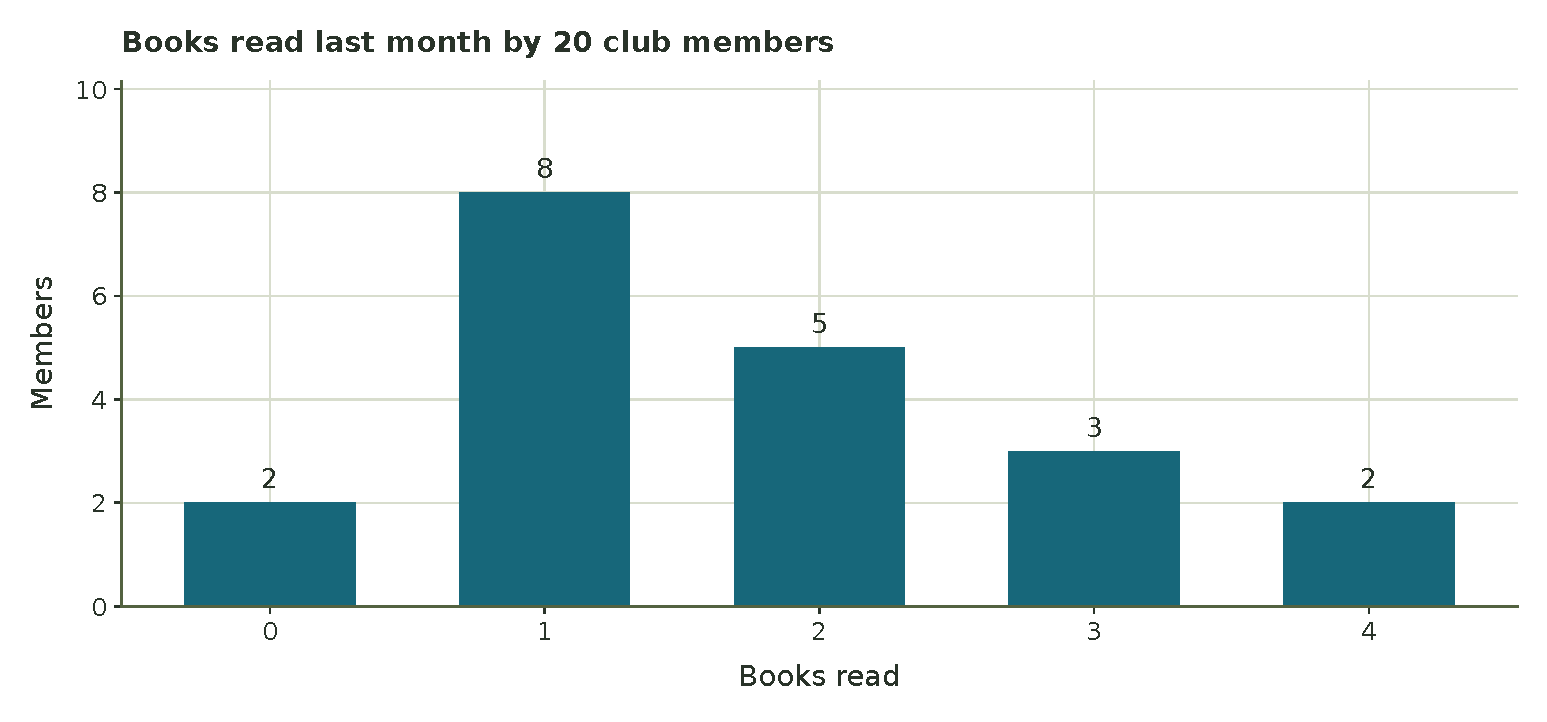
\includegraphics[width=\linewidth,height=2.6in,keepaspectratio]{../assets/week2/book-club.pdf}\end{center}
\item Forty office workers report their preferred lunch location: cafeteria 18, restaurant 10, desk 8, outside 4. Draw a bar chart of relative frequencies and identify the most and least common preferences.
\end{enumerate}

\Needspace{8\baselineskip}
\section*{Practice E: Histograms}
Use the stated left-closed, right-open bins: [a,b) includes a and excludes b.
\begin{enumerate}[label=E\arabic*.,leftmargin=2.5em,itemsep=10pt]
\item The ages of 24 volunteers are
\begin{quote}22, 25, 31, 28, 35, 22, 29, 40, 33, 27, 25, 38, 30, 26, 42, 23, 31, 29, 35, 24, 27, 33, 28, 36.\end{quote}
Group the ages into [20,25), [25,30), [30,35), [35,40), [40,45). Construct a frequency table, draw a relative-frequency histogram, and identify the bin with the greatest count.
\item Use the weekly social-media-hours histogram below. How many students are represented? What is the relative frequency of [10,15) hours? Describe its shape and justify your answer.
\begin{center}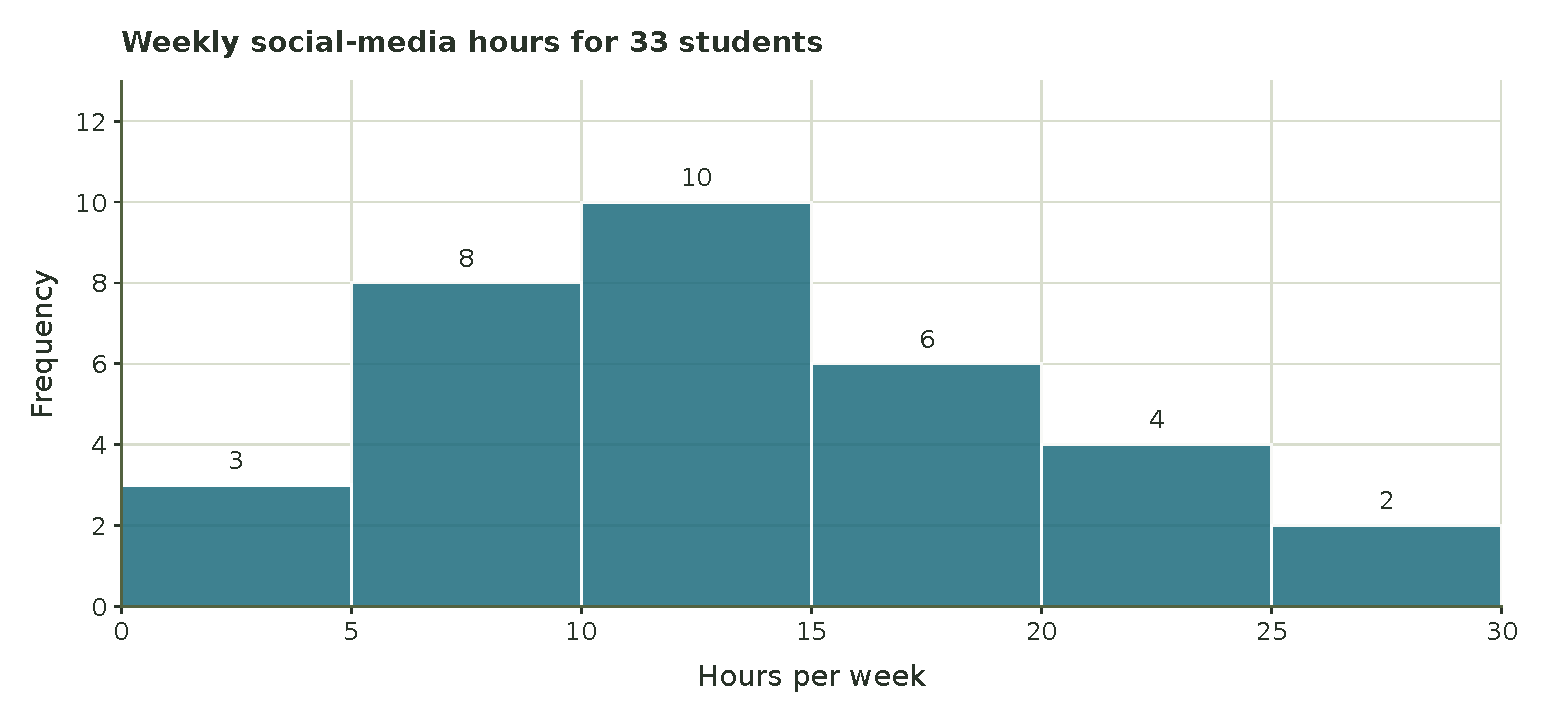
\includegraphics[width=\linewidth,height=2.7in,keepaspectratio]{../assets/week2/social-hours.pdf}\end{center}
\item Explain the difference between a bar chart and a histogram. Give one appropriate example for each.
\end{enumerate}

\Needspace{8\baselineskip}
\section*{Practice F: Probability distributions}
\begin{enumerate}[label=F\arabic*.,leftmargin=2.5em,itemsep=10pt]
\item Decide whether each complete list is a valid probability distribution. Explain any failure.
\begin{enumerate}[label=(\alph*)]
\item A, B, C with probabilities 0.3, 0.5, 0.2.
\item A, B, C with probabilities 0.4, 0.4, 0.4.
\item A, B with probabilities 0.7 and $-0.3$.
\item A, B, C, D with probabilities 0.25 each.
\end{enumerate}
\item A bag has 3 red, 4 blue, and 5 green chips. Each chip is equally likely to be drawn. Construct the color distribution, draw a bar chart, and find P(not blue).
\item For two fair independent six-sided dice, find P(sum $\leq6$) and P(sum $\geq8$). Explain why they are equal.
\item The number of errors in a randomly selected document has the distribution below.
\begin{center}\begin{tabular}{lrrrrr}\toprule
Errors & 0 & 1 & 2 & 3 & 4\\
Probability & .50 & .30 & .12 & .05 & .03\\\bottomrule
\end{tabular}\end{center}
Verify the distribution. Find P(at least one error). Sketch its numerical probability display using equal-width bars centered at the integer error counts. Describe its shape.
\end{enumerate}

\Needspace{8\baselineskip}
\section*{Chapter 2 Review}
\begin{enumerate}[label=R\arabic*.,leftmargin=2.5em,itemsep=10pt]
\item A team inspects 50 products: 0 defects for 28 items, 1 defect for 14, 2 defects for 6, and 3 defects for 2. Construct frequency and relative-frequency tables. Draw a histogram with width-one bins centered at the integer defect counts. Find the probability that a uniformly chosen inspected item has at least one defect. Describe the shape.
\item Sixty commuters have recorded travel times: [0,15) minutes, 12 commuters; [15,30), 22; [30,45), 18; [45,60), 8. Construct a relative-frequency table and histogram. Find the share with travel time at least 15 and less than 45 minutes.
\item A spinner's first three section probabilities are $1/3$, $1/4$, and $1/6$. Find the fourth probability p. Find the probability of one of the first two sections.
\item Explain in two sentences the difference between empirical and theoretical probability distributions, giving an example of each.
\item Thirty students report last night's sleep: 4 hours for 2 students, 5 for 4, 6 for 8, 7 for 10, 8 for 5, and 9 for 1. Construct a relative-frequency table and histogram with width-one bins centered at the reported hours. Describe the shape, a rough center, and the observed spread. Find the probability that a uniformly chosen student from this group slept fewer than 7 hours.
\item An administrator uses one advisory class to describe a school of 400 students, with 100 in each of four grade levels. The advisory has 20 students, all seniors. Identify population and sample. Explain in two sentences what the selection leaves out.
\end{enumerate}

\clearpage\section*{Solutions and reasoning}

\paragraph{Short check 1.}
The population is all visits during that month. The sample is the recorded Friday-afternoon visits. Other days and times are missing, so their patterns may be underrepresented.


\paragraph{Short check 2.}
Red occurs 3 times, blue 2 times, and green 1 time. The total is 3 + 2 + 1 = 6 responses.


\paragraph{Short check 3.}
8/40 = 1/5 = 0.20 = 20\%. The count is 8; the share is 0.20.


\paragraph{Short check 4.}
Neither. Both shares equal 0.60, or 60\%, even though the second survey has twice as many yes answers and twice as many responses.


\paragraph{Short check 5.}
Use a bar chart for the separate lunch-location categories. Use a histogram for the numerical travel-time intervals.


\paragraph{Short check 6.}
29 goes in [25,30), 30 in [30,35), and 35 in [35,40). Each value is counted once.


\paragraph{Short check 7.}
No. The model probability is 1/6; this sample's relative frequency is 1/12. A small sample does not have to match the model exactly.


\paragraph{Short check 8.}
No. They add to 1.10, which assigns more than the whole probability. Nonnegative entries alone are not enough.


\paragraph{Short check 9.}
P(1 or 2) = 2/6 = 1/3. The complement has probability 1 $-$ 1/3 = 2/3, covering 3, 4, 5, and 6.


\paragraph{Short check 10.}
The pairs are (5,6) and (6,5). The probability is 2/36 = 1/18. Of the 36 equally likely pairs, two have sum 11.


\paragraph{Short check 11.}
The expected count is 50 $\times$ 0.10 = 5. A particular run can have a different count.


\paragraph{Short check 12.}
40\% can be the largest category without being a majority; a majority means more than 50\%. We would need to know the population being studied, how respondents were selected, and who was left out or did not answer.


\clearpage

\Needspace{8\baselineskip}\subsection*{Practice A: Populations and samples}
\begin{enumerate}[label=A\arabic*.,leftmargin=2.5em,itemsep=10pt]
\item (a) The population is all ER patients during the month; the sample is the patients recorded last Tuesday. Other days and times may have different workloads or wait times. (b) The population is all registered voters in the group of interest; the selected sample is the 1,000 registered voters. Random selection gives voters a chance to be included, but unavailable phone numbers or nonresponse can still change who actually answers. (c) The intended population is the coffee shop\textquotesingle s customers; the sample is the Monday-morning customers who answer. People visiting at other times are missed, and current morning visitors may have different preferences.
\item From a complete list of the city\textquotesingle s teenagers, randomly select a fixed number of different names so every group of that size has the same chance. Survey those selected and record nonresponses. Asking only members of an online gaming club would favor teenagers who participate in that club and could overrepresent particular screen-use patterns.
\item A larger sample collected by the same limited method can repeat the same omission many more times. It gives more information about the people that method reaches, without automatically supplying information about the people it misses.
\end{enumerate}

\Needspace{8\baselineskip}\subsection*{Practice B: Frequency tables}
\begin{enumerate}[label=B\arabic*.,leftmargin=2.5em,itemsep=10pt]
\item \par\medskip{\small\renewcommand{\arraystretch}{1.25}\begin{tabularx}{\linewidth}[t]{@{}YYYY@{}}\toprule
Outcome & Frequency & Fraction & Decimal\\\midrule
{0} & 4 & $\frac{2}{9}$ & 0.2222\\
{1} & 7 & $\frac{7}{18}$ & 0.3889\\
{2} & 5 & $\frac{5}{18}$ & 0.2778\\
{3} & 2 & $\frac{1}{9}$ & 0.1111\\
Total & 18 & 1 & 1.0000\\\bottomrule\end{tabularx}}\par\medskip
The frequencies are 4, 7, 5, and 2, adding to 18. One sibling is the most common answer, occurring seven times.
\item \par\medskip{\small\renewcommand{\arraystretch}{1.25}\begin{tabularx}{\linewidth}[t]{@{}YYYY@{}}\toprule
Outcome & Frequency & Fraction & Decimal\\\midrule
{Car} & 10 & $\frac{1}{2}$ & 0.5000\\
{Bus} & 4 & $\frac{1}{5}$ & 0.2000\\
{Bike} & 3 & $\frac{3}{20}$ & 0.1500\\
{Walk} & 3 & $\frac{3}{20}$ & 0.1500\\
Total & 20 & 1 & 1.0000\\\bottomrule\end{tabularx}}\par\medskip
Car is most common, with 10 responses. The other methods account for $4+3+3=10$ employees.
\item The known counts total $8+12+5=25$. The missing category has $30-25=5$ observations.
\end{enumerate}

\Needspace{8\baselineskip}\subsection*{Practice C: Relative frequency and probability}
\begin{enumerate}[label=C\arabic*.,leftmargin=2.5em,itemsep=10pt]
\item \par\medskip{\small\renewcommand{\arraystretch}{1.25}\begin{tabularx}{\linewidth}[t]{@{}YYYY@{}}\toprule
Outcome & Frequency & Fraction & Decimal\\\midrule
{0} & 4 & $\frac{2}{9}$ & 0.2222\\
{1} & 7 & $\frac{7}{18}$ & 0.3889\\
{2} & 5 & $\frac{5}{18}$ & 0.2778\\
{3} & 2 & $\frac{1}{9}$ & 0.1111\\
Total & 18 & 1 & 1.0000\\\bottomrule\end{tabularx}}\par\medskip
The exact total is $(4+7+5+2)/18=1$. The chance of exactly one sibling, within this group, is $7/18\approx0.3889$. More than one sibling combines the counts for 2 and 3: $(5+2)/18=7/18\approx0.3889$. These happen to be equal in this dataset.
\item Each of the five equally sized sections has probability $1/5=0.20$. Not red has probability $4/5=0.80$. Red or orange has probability $2/5=0.40$. This assumes a fair spinner.
\item Outcomes 1, 2, 3, 4, 5, and 6 each have probability $1/6$. P(4) is $1/6$. P(even) is $3/6=1/2$, from 2, 4, 6. P(greater than 4) is $2/6=1/3$, from 5 and 6.
\item $p=1-(0.15+0.30+0.25)=0.30$. The listed outcomes cover all the probability, so their shares must sum to 1.
\end{enumerate}

\Needspace{8\baselineskip}\subsection*{Practice D: Bar charts}
\begin{enumerate}[label=D\arabic*.,leftmargin=2.5em,itemsep=10pt]
\item \par\medskip{\small\renewcommand{\arraystretch}{1.25}\begin{tabularx}{\linewidth}[t]{@{}YYYY@{}}\toprule
Outcome & Frequency & Fraction & Decimal\\\midrule
{Car} & 10 & $\frac{1}{2}$ & 0.5000\\
{Bus} & 4 & $\frac{1}{5}$ & 0.2000\\
{Bike} & 3 & $\frac{3}{20}$ & 0.1500\\
{Walk} & 3 & $\frac{3}{20}$ & 0.1500\\
Total & 20 & 1 & 1.0000\\\bottomrule\end{tabularx}}\par\medskip

\par\medskip\noindent\begin{minipage}{\linewidth}\centering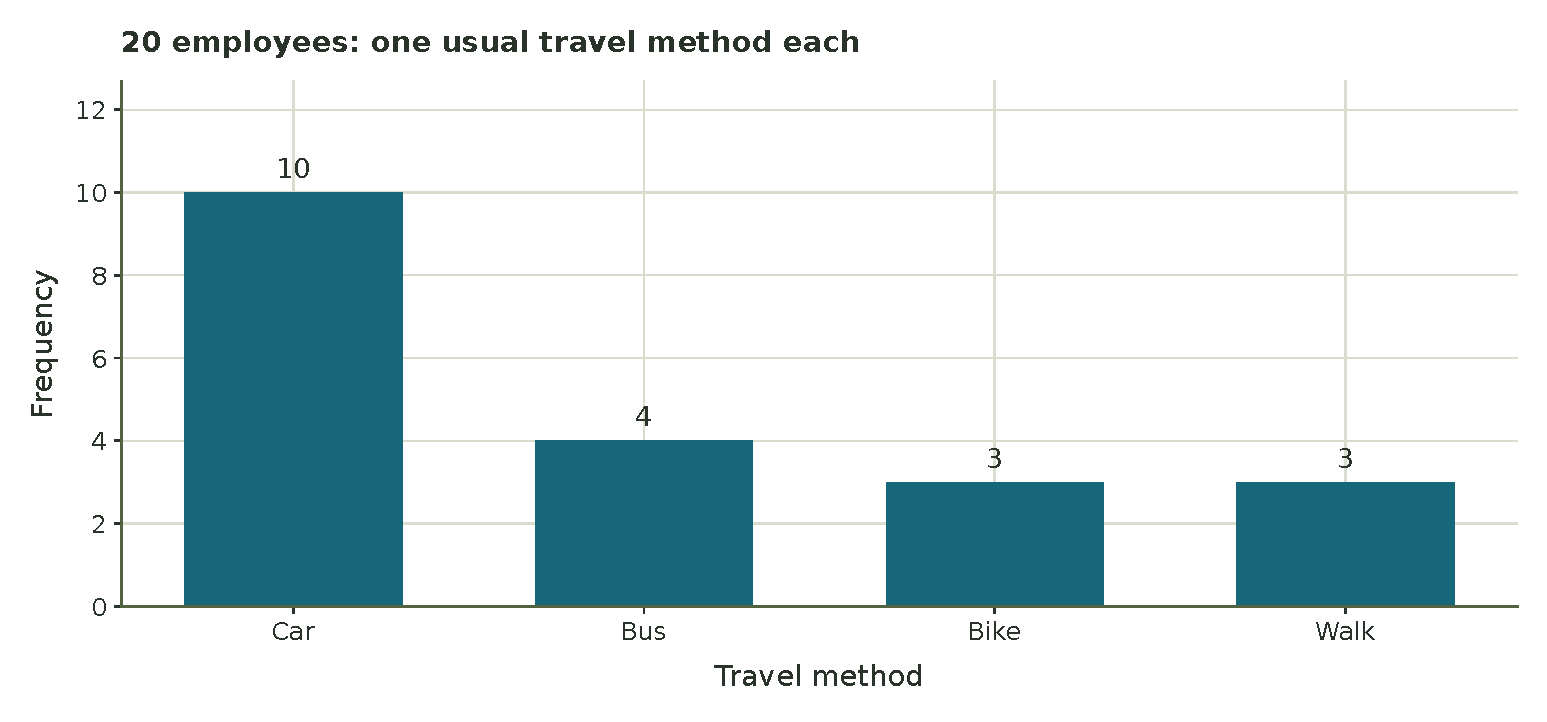
\includegraphics[width=\linewidth,height=2.6in,keepaspectratio]{../assets/week2/employee-transport.pdf}\captionof*{figure}{For a relative-frequency version, use bar heights 0.50, 0.20, 0.15, and 0.15 instead of the raw counts.}\end{minipage}\par\medskip
Any pair containing car and one other method exceeds half: car + bus is 0.70, car + bike is 0.65, and car + walk is 0.65. No pair without car exceeds half. There is more than one correct pair.
\item The total is $2+8+5+3+2=20$ members. Exactly one book gives $8/20=0.40$. More than two books combines 3 and 4: $(3+2)/20=0.25$.
\item \par\medskip{\small\renewcommand{\arraystretch}{1.25}\begin{tabularx}{\linewidth}[t]{@{}YYYY@{}}\toprule
Outcome & Frequency & Fraction & Decimal\\\midrule
{Cafeteria} & 18 & $\frac{9}{20}$ & 0.4500\\
{Restaurant} & 10 & $\frac{1}{4}$ & 0.2500\\
{Desk} & 8 & $\frac{1}{5}$ & 0.2000\\
{Outside} & 4 & $\frac{1}{10}$ & 0.1000\\
Total & 40 & 1 & 1.0000\\\bottomrule\end{tabularx}}\par\medskip

\par\medskip\noindent\begin{minipage}{\linewidth}\centering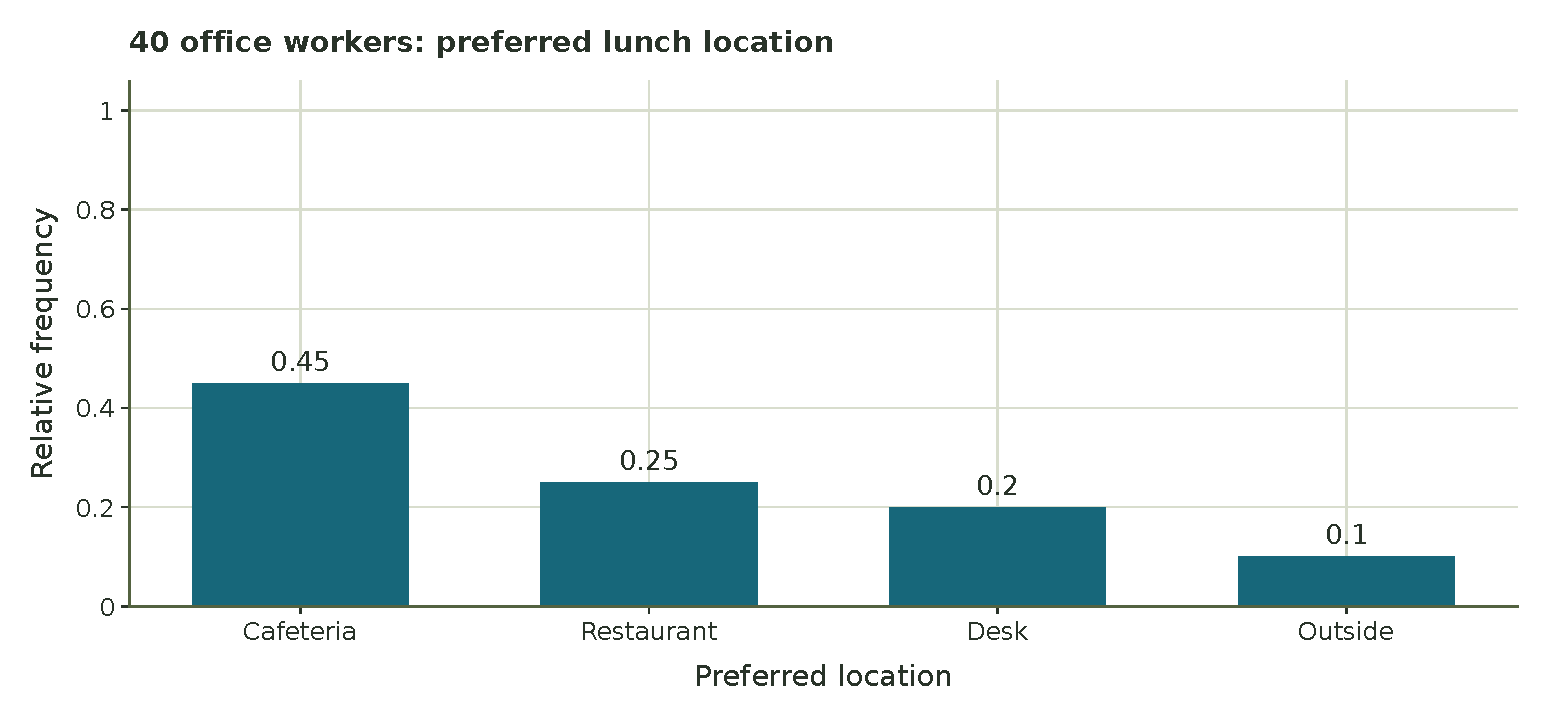
\includegraphics[width=\linewidth,height=2.6in,keepaspectratio]{../assets/week2/lunch-locations.pdf}\captionof*{figure}{Cafeteria is the most common preference; outside is the least common. The vertical axis shows shares, not counts.}\end{minipage}\par\medskip

\end{enumerate}

\Needspace{8\baselineskip}\subsection*{Practice E: Histograms}
\begin{enumerate}[label=E\arabic*.,leftmargin=2.5em,itemsep=10pt]
\item \par\medskip{\small\renewcommand{\arraystretch}{1.25}\begin{tabularx}{\linewidth}[t]{@{}YYYY@{}}\toprule
Outcome & Frequency & Fraction & Decimal\\\midrule
{[20,25)} & 4 & $\frac{1}{6}$ & 0.1667\\
{[25,30)} & 9 & $\frac{3}{8}$ & 0.3750\\
{[30,35)} & 5 & $\frac{5}{24}$ & 0.2083\\
{[35,40)} & 4 & $\frac{1}{6}$ & 0.1667\\
{[40,45)} & 2 & $\frac{1}{12}$ & 0.0833\\
Total & 24 & 1 & 1.0000\\\bottomrule\end{tabularx}}\par\medskip

\par\medskip\noindent\begin{minipage}{\linewidth}\centering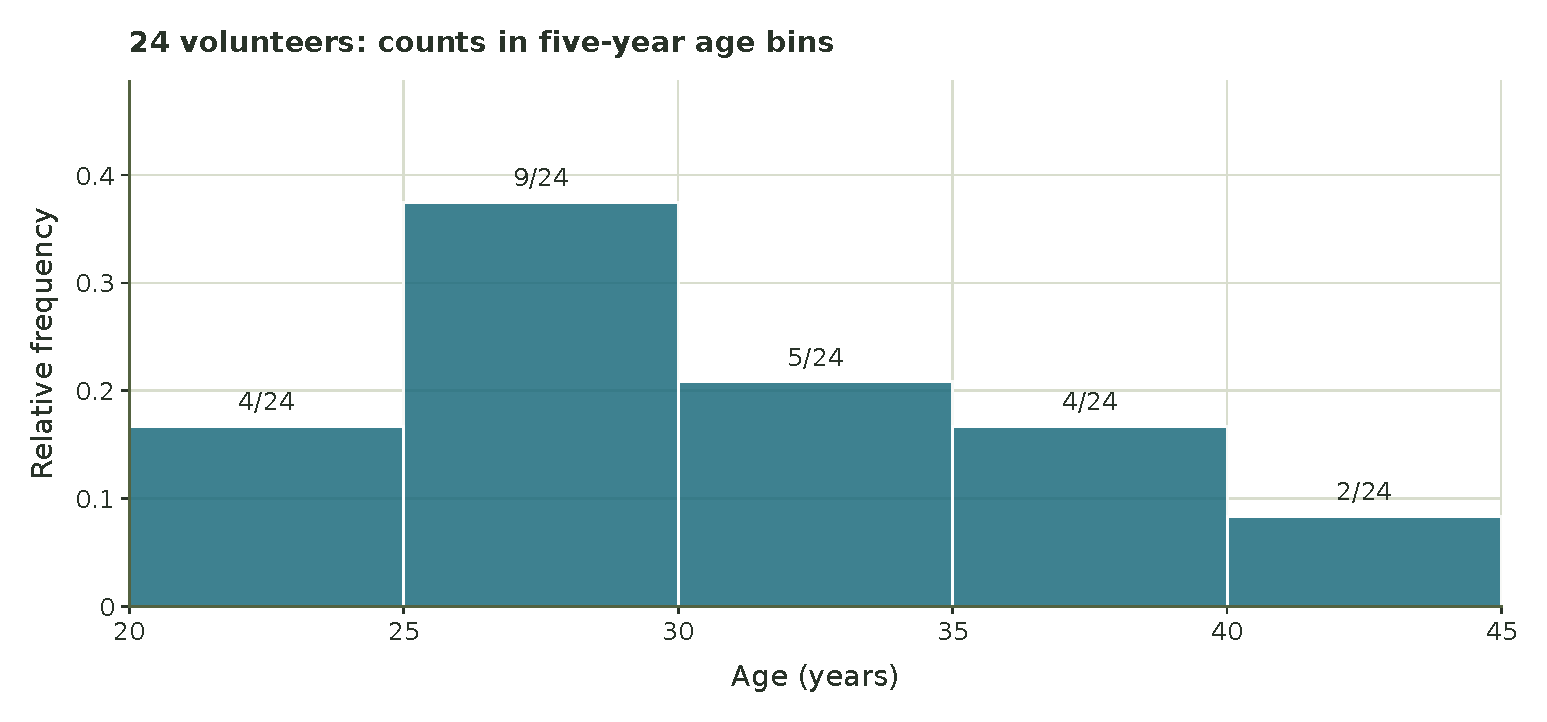
\includegraphics[width=\linewidth,height=2.6in,keepaspectratio]{../assets/week2/volunteer-ages.pdf}\captionof*{figure}{The largest bin is [25,30), with 9 of 24 observations: 0.375, or 37.5\%.}\end{minipage}\par\medskip
The age 25 goes in the second bin, not the first. The five bin counts total 24.
\item The counts total $3+8+10+6+4+2=33$. The [10,15) bin has share $10/33\approx0.3030$. The display is somewhat skewed right: after the main cluster near 10--15 hours, the small bars extend farther toward larger hours than toward smaller hours.
\item A bar chart compares separate categories, such as preferred study locations, using separate bars. A histogram groups numerical measurements into ordered intervals, such as commute time in 15-minute bins, with adjacent bars touching.
\end{enumerate}

\Needspace{8\baselineskip}\subsection*{Practice F: Probability distributions}
\begin{enumerate}[label=F\arabic*.,leftmargin=2.5em,itemsep=10pt]
\item (a) Valid: entries are between 0 and 1 and sum to 1. (b) Invalid: the sum is 1.2. (c) Invalid: one probability is negative; the sum is also only 0.4. (d) Valid: four entries of 0.25 sum to 1.
\item \par\medskip{\small\renewcommand{\arraystretch}{1.25}\begin{tabularx}{\linewidth}[t]{@{}YYYY@{}}\toprule
Outcome & Frequency & Fraction & Decimal\\\midrule
{Red} & 3 & $\frac{1}{4}$ & 0.2500\\
{Blue} & 4 & $\frac{1}{3}$ & 0.3333\\
{Green} & 5 & $\frac{5}{12}$ & 0.4167\\
Total & 12 & 1 & 1.0000\\\bottomrule\end{tabularx}}\par\medskip

\par\medskip\noindent\begin{minipage}{\linewidth}\centering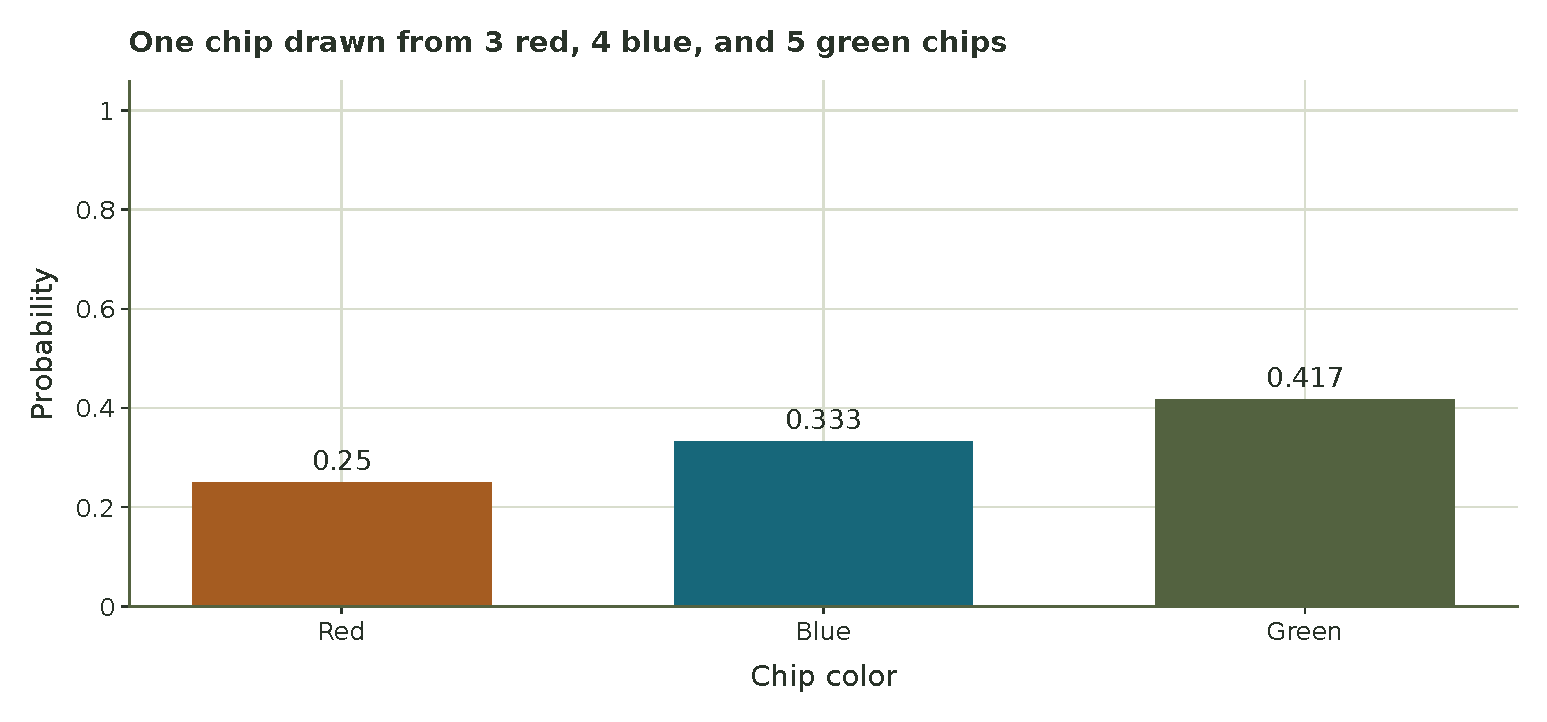
\includegraphics[width=\linewidth,height=2.6in,keepaspectratio]{../assets/week2/chip-distribution.pdf}\captionof*{figure}{The probabilities are 1/4, 1/3, and 5/12, based on equally likely individual chips.}\end{minipage}\par\medskip
P(not blue) $=1-4/12=8/12=2/3$. Red and green together give the same result: $(3+5)/12=2/3$.
\item Sums 2 through 6 account for $1+2+3+4+5=15$ of the 36 equally likely pairs, so P(sum $\leq6$) $=15/36=5/12$. Sums 8 through 12 also account for $5+4+3+2+1=15$ pairs. Symmetry around 7 explains the equality. The six pairs summing to 7 belong to neither event.
\item All entries lie between 0 and 1, and $0.50+0.30+0.12+0.05+0.03=1$. P(at least one error) $=1-P(0)=0.50$; adding the four positive-error probabilities also gives 0.50.
\par\medskip\noindent\begin{minipage}{\linewidth}\centering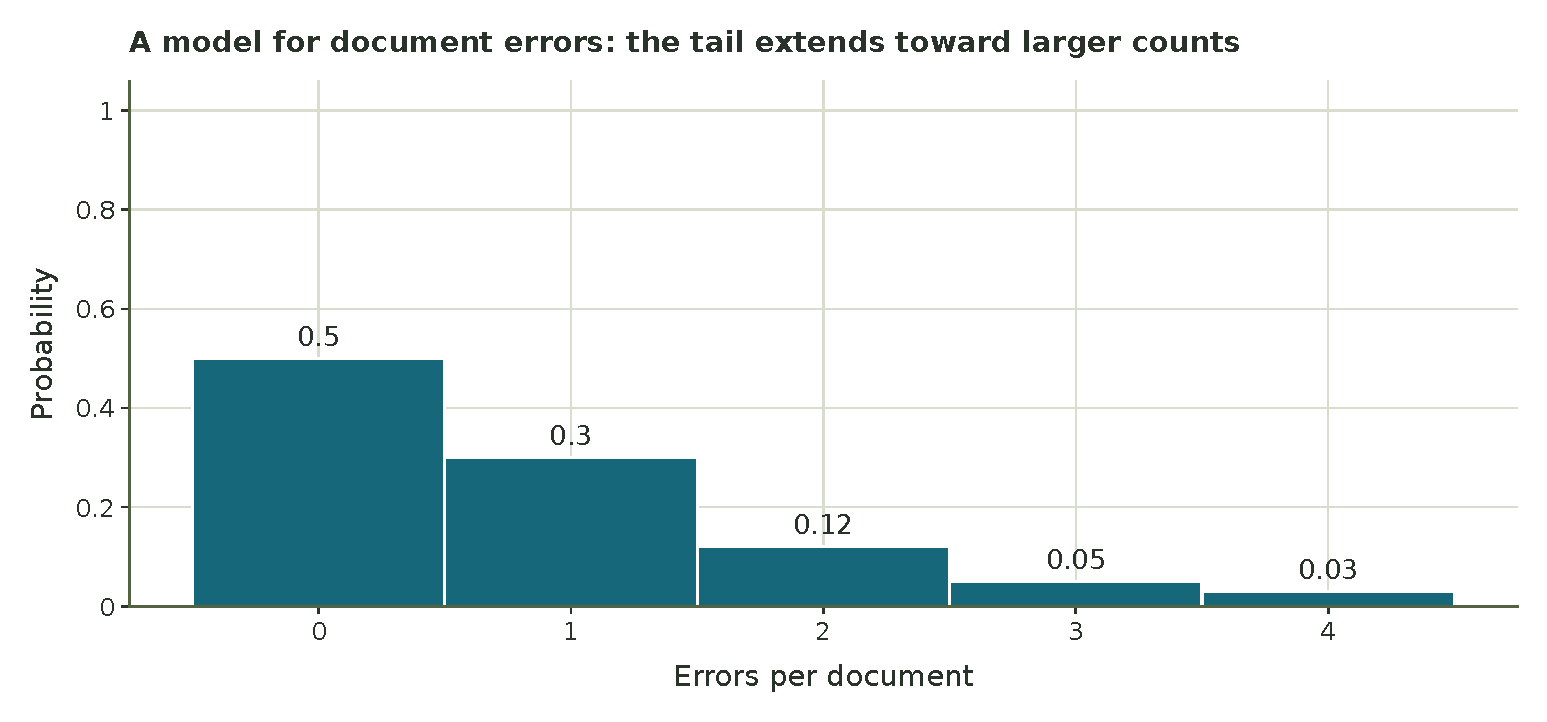
\includegraphics[width=\linewidth,height=2.6in,keepaspectratio]{../assets/week2/document-errors.pdf}\captionof*{figure}{The tail extends toward larger error counts, so this display is skewed right.}\end{minipage}\par\medskip

\end{enumerate}

\Needspace{8\baselineskip}\subsection*{Chapter 2 review}
\begin{enumerate}[label=R\arabic*.,leftmargin=2.5em,itemsep=10pt]
\item \par\medskip{\small\renewcommand{\arraystretch}{1.25}\begin{tabularx}{\linewidth}[t]{@{}YYYY@{}}\toprule
Outcome & Frequency & Fraction & Decimal\\\midrule
{0} & 28 & $\frac{14}{25}$ & 0.5600\\
{1} & 14 & $\frac{7}{25}$ & 0.2800\\
{2} & 6 & $\frac{3}{25}$ & 0.1200\\
{3} & 2 & $\frac{1}{25}$ & 0.0400\\
Total & 50 & 1 & 1.0000\\\bottomrule\end{tabularx}}\par\medskip

\par\medskip\noindent\begin{minipage}{\linewidth}\centering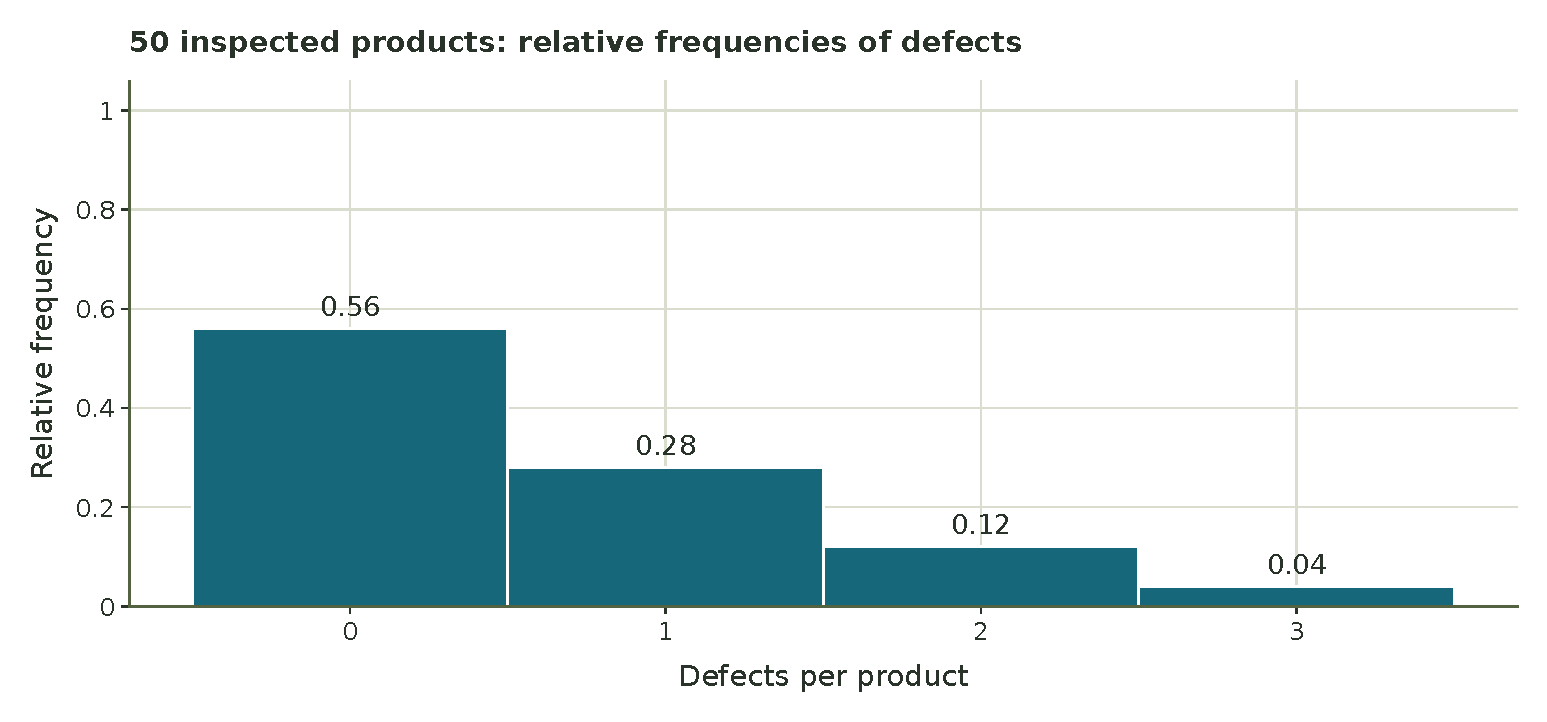
\includegraphics[width=\linewidth,height=2.6in,keepaspectratio]{../assets/week2/quality-defects.pdf}\captionof*{figure}{Width-one bins are centered at the integer defect counts. Most items have no defects; small bars extend toward larger counts.}\end{minipage}\par\medskip
P(at least one defect) $=1-28/50=22/50=0.44$. The distribution is skewed right.
\item \par\medskip{\small\renewcommand{\arraystretch}{1.25}\begin{tabularx}{\linewidth}[t]{@{}YYYY@{}}\toprule
Outcome & Frequency & Fraction & Decimal\\\midrule
{[0,15)} & 12 & $\frac{1}{5}$ & 0.2000\\
{[15,30)} & 22 & $\frac{11}{30}$ & 0.3667\\
{[30,45)} & 18 & $\frac{3}{10}$ & 0.3000\\
{[45,60)} & 8 & $\frac{2}{15}$ & 0.1333\\
Total & 60 & 1 & 1.0000\\\bottomrule\end{tabularx}}\par\medskip

\par\medskip\noindent\begin{minipage}{\linewidth}\centering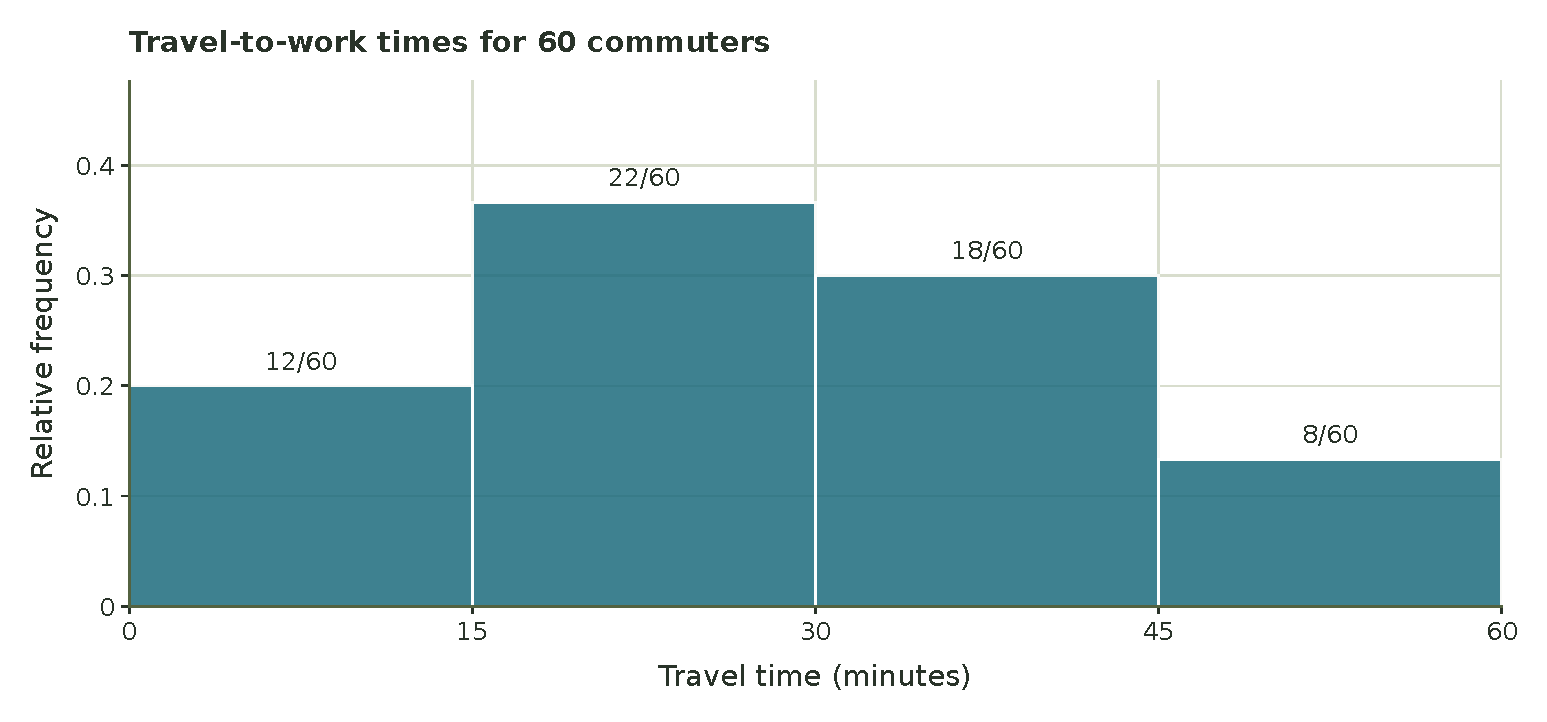
\includegraphics[width=\linewidth,height=2.6in,keepaspectratio]{../assets/week2/commute-review.pdf}\captionof*{figure}{All bins are 15 minutes wide. Their heights show relative frequencies.}\end{minipage}\par\medskip
At least 15 and less than 45 minutes combines the middle two bins: $(22+18)/60=40/60=2/3\approx0.6667$. The stated endpoint rule includes 15 and excludes 45.
\item The three known probabilities total $1/3+1/4+1/6=4/12+3/12+2/12=9/12=3/4$. Therefore $p=1/4$. The first two sections have combined probability $1/3+1/4=7/12$.
\item An empirical distribution comes from observed counts, such as the proportions of 80 surveyed workers using different commuting methods. A theoretical distribution comes from model assumptions, such as assigning each face of a fair die probability 1/6.
\item \par\medskip{\small\renewcommand{\arraystretch}{1.25}\begin{tabularx}{\linewidth}[t]{@{}YYYY@{}}\toprule
Outcome & Frequency & Fraction & Decimal\\\midrule
{4} & 2 & $\frac{1}{15}$ & 0.0667\\
{5} & 4 & $\frac{2}{15}$ & 0.1333\\
{6} & 8 & $\frac{4}{15}$ & 0.2667\\
{7} & 10 & $\frac{1}{3}$ & 0.3333\\
{8} & 5 & $\frac{1}{6}$ & 0.1667\\
{9} & 1 & $\frac{1}{30}$ & 0.0333\\
Total & 30 & 1 & 1.0000\\\bottomrule\end{tabularx}}\par\medskip

\par\medskip\noindent\begin{minipage}{\linewidth}\centering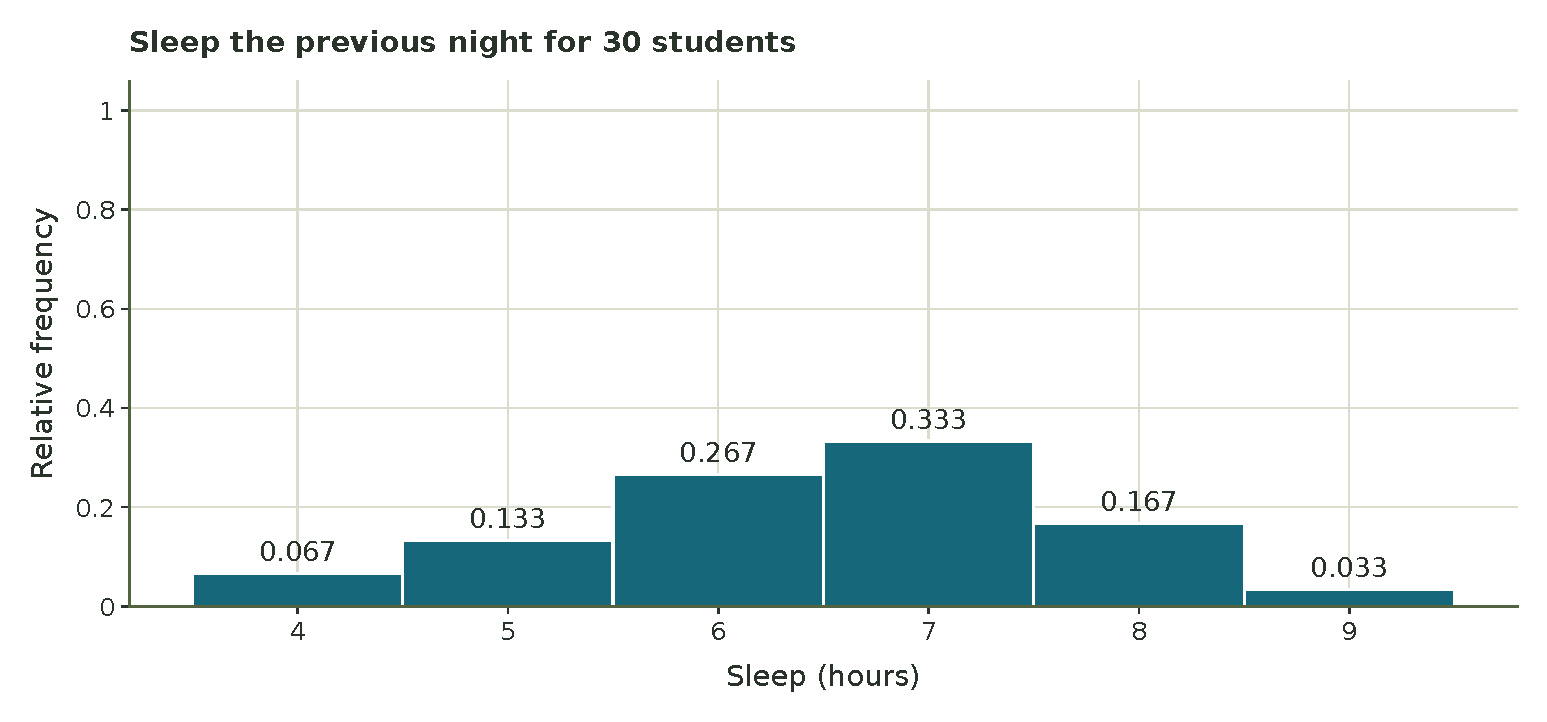
\includegraphics[width=\linewidth,height=2.6in,keepaspectratio]{../assets/week2/sleep-review.pdf}\captionof*{figure}{Most observations lie around 6--7 hours, with reported values from 4 through 9 hours.}\end{minipage}\par\medskip
The shape is roughly mound-like, with a slightly longer tail toward the lower hours. A rough center is around 6--7 hours; the observed span is 4--9 hours. This description does not require the formal mean or standard deviation introduced next week. Fewer than 7 hours combines 4, 5, and 6: $(2+4+8)/30=14/30=7/15\approx0.4667$.
\item The population is all 400 students; the sample is the 20 students in that advisory. Every sampled student is a senior, while only 100 of 400 students in the school are seniors. The sample leaves out the other 300 students in three grade levels, so it cannot directly reveal their views.
\end{enumerate}

\end{document}
